%% $RCSfile: proj_report_outline.tex,v $
%% $Revision: 1.3 $
%% $Date: 2016/06/10 03:41:54 $
%% $Author: kevin $

\documentclass[11pt
              , a4paper
              , twoside
              , openright
              ]{report}


\usepackage{float} % lets you have non-floating floats

\usepackage{url} % for typesetting urls
\usepackage{xcolor}
\usepackage{tikz}
\usepackage{amsmath}
\usepackage{bm}
\usepackage{algorithm}
\usepackage{algpseudocode}
\usepackage{hyperref}
\usepackage{float}
\usepackage{booktabs} 
\usepackage{tabularx} % Add this to the preamble

%
%  We don't want figures to float so we define
%
\newfloat{fig}{thp}{lof}[chapter]
\floatname{fig}{Figure}

%% These are standard LaTeX definitions for the document
%%                            
\title{Reinforcement Learning \\
\large Part 3: Complete report of current Reinforcement algorithms and a new algorithm with evaluations}

\author{James Thompson}

%% This file can be used for creating a wide range of reports
%%  across various Schools
%%
%% Set up some things, mostly for the front page, for your specific document
%
% Current options are:
% [ecs|msor|sms]          Which school you are in.
%                         (msor option retained for reproducing old data)
% [bschonscomp|mcompsci]  Which degree you are doing
%                          You can also specify any other degree by name
%                          (see below)
% [font|image]            Use a font or an image for the VUW logo
%                          The font option will only work on ECS systems
%
\usepackage[font,ecs]{vuwproject}

% You should specifiy your supervisor here with
%     \supervisor{Firstname Lastname}
% use \supervisors if there is more than one supervisor
\supervisor{Dr Aaron Chen}

% Unless you've used the bschonscomp or mcompsci
%  options above use
%   \otherdegree{OTHER DEGREE OR DIPLOMA NAME}
% here to specify degree
\otherdegree{Master of Artificial Intelligence}

% Comment this out if you want the date printed.
\date{\today}

\begin{document}

% Make the page numbering roman, until after the contents, etc.
\frontmatter

%%%%%%%%%%%%%%%%%%%%%%%%%%%%%%%%%%%%%%%%%%%%%%%%%%%%%%%

%%%%%%%%%%%%%%%%%%%%%%%%%%%%%%%%%%%%%%%%%%%%%%%%%%%%%%%

\begin{abstract}
This is submitted for the completion of AIML440 Directed individual study as part of the Master of Artificial Intelligence programme at Victoria University of Wellington. This report has three sections. Firstly an Introduction of reinforcement learning and basic algorithms. Secondly I will evaluate modern algorithms. Lastly I propose a new algorithm Dynamic-Sunrise (DSunrise) which is an extension of Sunrise that maintains the diversity of the ensemble throughout learning.
\end{abstract}

%%%%%%%%%%%%%%%%%%%%%%%%%%%%%%%%%%%%%%%%%%%%%%%%%%%%%%%

\maketitle

% Removed because I have no acknowledgements
% \chapter*{Acknowledgments}\label{C:ack} 
Any acknowledgments should go 
in here, between the title page and the table of contents.  The 
acknowledgments do not form a proper chapter, and so don't get a 
number or appear in the table of contents.

\tableofcontents

% we want a list of the figures we defined
% \listof{fig}{Figures}

%%%%%%%%%%%%%%%%%%%%%%%%%%%%%%%%%%%%%%%%%%%%%%%%%%%%%%%

\mainmatter

%%%%%%%%%%%%%%%%%%%%%%%%%%%%%%%%%%%%%%%%%%%%%%%%%%%%%%%

% individual chapters included here

\chapter{Introduction}\label{C:intro}

\subsection{The reinforcement learning problem}

Reinforcement learning is a framework that describes how an agent learns by interacting with the environment. The framework involves 2 entities the agent and environment. The agent is the only entity that we as designers have direct control of. We decide how its learns and decides on its actions. The environment is the context and situation that the agent is in. There are three important flows of information;  the state of the environment to the agent, the action decision to the environment and lastly the reward to the agent. This can be best be understood in the figure below.

\begin{fig}
\begin{center}
    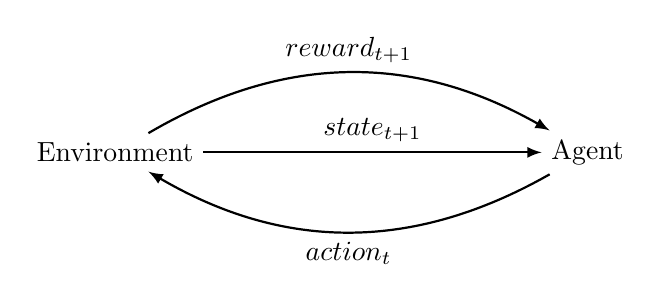
\begin{tikzpicture}[
        node distance=6cm, % Increased node distance for better spacing
    ]
        % Define nodes
        \node (env) {Environment};
        \node (agent) [right of=env] {Agent};

        % Define arrows and labels without boxes
        \draw [-latex,bend left, thick] (env) edge node[anchor=south] {$reward_{t+1}$} (agent);
        \draw [-latex, thick] (env) -- node[anchor=south] {$state_{t+1}$} (agent);
        \draw [-latex,bend left,thick] (agent) edge node[anchor=north] {$action_{t}$} (env);
    \end{tikzpicture}
    \caption{The flow of information between th environment and agent}
\end{center}
\end{fig}

The state is a representation of the information within the environment that the agent observes to make its decision on which action to take. The reward signal is treated as the final word on how good the previous state action was, the more reward the better, always. Lastly the action taken by the agent is sent to the environment and the environment will in turn return the next state and reward. This brings us to the reinforcement learning problem which can be framed as such "How does the agent decide which actions to take given the state such that it maximises the future cumulative reward". It is important that the agent maximises all \textit{future cumulative} reward otherwise short term gains could be made to the sacrifice of larger long term gains. This idea has been formalised by Richard Sutton as the reward hypothesis

\begin{quote}
    "That all of what we mean by goals and purposes can be well thought of as maximization of the expected value of the cumulative sum of a received scalar signal (reward)." 
    \cite{suttonReinforcementLearningSecond2018}
    \label{quote:reward}
\end{quote}

\subsection{Formalism}

The reinforcement problem can be formalised as a Markov Decision Process (MDP). The MDP is a collection of states, actions and rewards along with a transition function which states the probability of the next reward and state given a state and reward. This makes the MDP a 4-tuple $(S,\mathcal{A}, \mathcal{P}, R)$ where $S$ is the set of states, $\mathcal{A}(s)$ is the set of actions that can be taken from state $s$, $\mathcal{P}$ is the transition function and $R \subset \mathbb{R}$ is the set of rewards. The transition function is defined as:

\begin{equation}
\mathcal{P}(s',r, s,a) = Pr\left\{ S_{t}=s', R_{t}=r | S_{t-1}=s, A_{t-1}=a \right\}
\label{eq:transition}
\end{equation}
Where $s,s \in S, a \in \mathcal{A}(s) \text{ and } r \in R$.

This transition function completely characterises the dynamics of the environment. The abstraction of the environment to a MDP is widely applicable and serves as the basis for much of reinforcement learning. We can see here that transition function only looks at the previous state. It can do this because we assume that the state representation has the \textit{Markov property} \cite{suttonReinforcementLearningSecond2018}. The Markov property states that including previous states in the conditional wont change the probability of next state reward tuple. In other words $\mathcal{P}(s_{t+1}, r_{t+1}, s_{t},a_{t}) = \mathcal{P}(s_{t+1}, r_{t+1}, s_{t},a_{t}, s_{t-1}, s_{t-2}, ... , s_{0})$. Therefore a state with the Markov property is a sufficient representation of the history of the agent-environment interaction. In some problems the agent only partially observes the state meaning the Markov property is not satisfied. This is called a partially observable MDP (POMDP) and is a more complex problem to solve which wont be addressed in this report.

The agent interacts with the MDP to produce a trajectory of states, actions and rewards. Because the agent will not know the transition function \ref{eq:transition} it will have to learn about the MDP from the information in a trajectory \ref{eq:MDPsequence}.

\begin{equation}
S_{1},A_{1},R_{2},\dots S_{n},A_{n}, R_{n+1},\dots 
\label{eq:MDPsequence}
\end{equation}

In this trajectory \ref{eq:MDPsequence} we have an infinite sequence as this is an example from a continuing MDP that has no end. Alternatively you could have episodic MDPs that have a start and end with a terminal state. Episodic MDPs require practical considerations in implementing algorithms. However for most of the theory it make no difference as you can think of a episode MDP as a continuing MPD with a state that transitions to itself and gives reward 0.

"The cumulative sum of a received scalar signal" part of the reward hypothesis \ref{quote:reward} can be formalised to be the return $G$.

\begin{equation}
G_{t}=R_{t+1}+\gamma R_{t+2}+\gamma^{2}R_{t+3}\dots=\sum_{k=t}^{\infty}\gamma^{t-1}R_{t+1}
\end{equation}

$\gamma$ is called the discounting factor and weights future rewards to have less effect on the return. It is usually added for two reasons. Firstly because it makes the return finite which simplifies the mathematics. Secondly is due to the very natural intuition that the future is less predicable than the present, thus more distance rewards should have less weight as they are less certain. 


A agent will use policy $\pi$ which provides the probability of taking action $a$ given state $s$. This policy could be deterministic or stochastic.
To evaluate how good a policy is or how much reward we can expect at a state we need a function to tell us. This is called the value function and it is a expectation of the future rewards.

\begin{equation}
v_{\pi}(s)=\mathbb{E}\left[ G_{t}| S_{t}=s\right] 
\end{equation}

The state value function depends on the state, policy and discounting factor $\gamma$ which is used by the return. In a similar vain to the state value function we have the action-value function which is the expected future reward given a state and action taken.

\begin{equation}
q_{\pi}(s,a) = \mathbb{E}\left[ G_{t} | S_{t}=s, A_{t}=a \right] 
\end{equation}

We can understand how to compute the expectation of the value function by looking at the Bellman equation \cite{suttonReinforcementLearningSecond2018}. The Bellman equation is based off the notion that the value of a situation should be the immediate reward you get plus the value of the situation you end up in. This can be written for the state value function as follows:

\begin{equation}
v_{\pi}(s)=\sum_{a}\pi(a|s)\sum_{s',r}p(s',r|s,a)\left[ r+\gamma v_{\pi}(s') \right]
\end{equation}
$\pi(a|s)$ is the probability of taking action $a$ given state $s$ and $p(s',r|s,a)$ is the transition function. This equation can be solved for $v_{\pi}$ by iterating over all states and actions until the value function converges. This is called the iterative policy evaluation and is a dynamic programming technique \cite{bellmanDynamicProgramming1957}.

The maximising part of the reinforcement problem can be solved by the finding optimal actions. We can define both $v_{\star}=\underset{ \pi }{ \text{max} }\ v_{\pi}(s)$ and $q_{\star}=\underset{ \pi }{ \text{max} }\ q_{\pi}(s,a)$ as the optimal value given optimal actions afterwards.
If we can find $q_{\star}$ then the problem is solved as we could make a policy $\pi_{\star}$ that is greedy with respect to $q_{\star}$. Two things stop this from being so simple. Firstly is that in many real problems we don't know the true transition function, therefore we either have to learn/approximate or learn the value/policies in a way that doesn't involve the transition function. Secondly is the computational complexity of iterating over all states and actions as well as all possible policies. This is called the curse of dimensionality and is a major problem in reinforcement learning. If we try to learn and transition funtion and come up with a model of the environment then we are using model based methods, alternatively we ignore the model and learn the value or policy directly and these are called model free methods. In the rest of the report we will be focusing on model free methods.

The form of explicitly learning a value function then implicitly getting actions from it is called value based methods. Alternatively you can learn the policy directly with policy based methods. The effectiveness of these methods depend heavily on how easy the value function or policy is to learn.

\chapter{Algorithms}\label{C:algorithms}

In the real world we don't get access to the transition function of the MDP. The agents only method to learn is through interacting with the environment. From this interaction we get a sample of the environment and must learn from it. Therefore stochastic learning methods must be used. Two learning ideas are core for many reinforcement learning algorithms. These are Monte Carlo \cite{suttonReinforcementLearningSecond2018} and Temporal Difference learning \cite{suttonTemporalCreditAssignment1984} \cite{suttonLearningPredictMethods1988}.

\section{Traditional algorithms}

\subsection{Value Based Methods}

As mentioned earlier value based method focus on learning a value function and from that function we can derive a policy. The action value function is more powerful as simply knowing the value of a state is not enough to make a decision. The action value function is defined as the expected return given a state and action. Thus all you need to do is take the action that gives you the maximum $Q$ value.


Monte Carlo learning works by estimating the value function as being the average return from that state.  A basic algorithm would look like this.

\begin{algorithm}
\caption{Monte Carlo Control with Exploring Starts}
\begin{algorithmic}[1]
\State Arbitrarily initialize $\pi(s) \in \mathcal{A}(s)$ and $Q(s,a) \in \mathbb{R}$
\State $\text{Returns}(S,A) \gets$ empty list
\For{each episode}
    \State Arbitrarily choose $S_0 \in \mathcal{S}, A_0 \in \mathcal{A}$
    \State Generate an episode by following $\pi$
    \State $G \gets 0$
    \For{each step of the episode $t = T-1, T-2, \dots, 0$}
        \State $G \gets \gamma G + R_{t+1}$
        \If{$(S_t, A_t)$ does not appear earlier in the episode}
            \State Append $G$ to $\text{Returns}(S_t, A_t)$
            \State $Q(S_t, A_t) \gets \text{average}(\text{Returns}(S_t, A_t))$
            \State $\pi(S_t) \gets \arg\max_{a} Q(S_t, a)$
        \EndIf
    \EndFor
\EndFor
\end{algorithmic}
\end{algorithm}

Because we need a well defined return Monte Carlo methods only work on episodic tasks. It will only update the states that it actually visits. This gives us the option of just exploring the state space area we are interested in learning about.

Temporal difference learning works different incrementally updating the value of a state with the received reward and the value of the next state \ref{eq:TDupdate}. As the update is using its own estimate it is \textit{bootstrapping}. Because of bootstrapping it can work with both episodic and continuing environments.

\begin{equation}
V(S_{t})=R_{t+1}+\gamma V(S_{t+1})
\label{eq:TDupdate}
\end{equation}

Below is a basic implementation of TD learning for a continuing environment, however it is easy to change it to episdoic by changing the loop to be over episodes.

\begin{algorithm}
\caption{TD(0)}
\begin{algorithmic}[1]
\State Initialize $Q(s,a)$ arbitrarily and set $Q(\text{terminal-state}) = 0$
\State Initialize $S$
\While{not converged}
    \State Take action $A$, observe $R$, $S'$
    \State Choose $A' \in \mathcal{A}(S')$ using policy derived from $Q$
    \State $Q(S,A) \gets Q(S,A) + \alpha \left[ R + \gamma Q(S', A') - Q(S,A) \right]$
    \State $S \gets S'$; $A \gets A'$
\EndWhile
\end{algorithmic}
\end{algorithm}

This particular update is known as TD(0) because it only looks one step into the future. However it can be generalised to be TD(n). One can see that if we had TD($\infty$) we would be back at Monte Carlo if working in episodic tasks.

The two methods of TD(n) and Monte carlo can be to get the best of both worlds using TD($\lambda$) methods \cite{suttonLearningPredictMethods1988}.


\subsection{Policy Based Methods}

A different way of the approaching the problem is by learning the policy directly without a learning a concept of how good a state is. The most common policy based method is called policy gradient methods \cite{suttonPolicyGradientMethods1999}. To use policy gradient methods you need to parametize the policy $\pi$ in any way as long as $\pi(a|s, \theta)$ is differentiable with respect to $\theta$.

The first of these policy gradient methods was the Reinforce algorithm \cite{williamsSimpleStatisticalGradientfollowing1992}. It is a Monte Carlo policy gradient method. The updates are made by moving the policy in the direction of the gradient of the log probability of the action taken. This works because it is proportional to the return which is given to use by the policy gradient theorem \cite{suttonPolicyGradientMethods1999}.

\begin{algorithm}
\caption{REINFORCE: Monte-Carlo Policy-Gradient Control (episodic) for $\pi_*$}
\begin{algorithmic}[1]
\Require A differentiable policy parameterization $\pi(a|s, \theta)$
\Require Step size $\alpha > 0$
\State Initialize policy parameter $\theta \in \mathbb{R}^d$ (e.g., to 0)
\Loop
  \State Generate an episode $S_0, A_0, R_1, \ldots, S_{T-1}, A_{T-1}, R_T$, following $\pi(\cdot|\cdot, \theta)$
  \For{$t = 0, 1, \ldots, T-1$}
    \State $G \leftarrow \sum_{k=t+1}^{T} \gamma^{k-t-1} R_k$
    \State $\theta \leftarrow \theta + \alpha \gamma^t G \nabla \ln \pi(A_t|S_t, \theta)$
  \EndFor
\EndLoop
\end{algorithmic}
\end{algorithm}

\subsection{Challenges of traditional methods}

There are main two issues with the simple methods of TD and Monte Carlo mentioned above. This is scalability and exploration.

Firstly with scalability we are storing the action value of a particular state in a large lookup table. This will immediately become a problem when dealing with large state or action spaces. Most real world application have tremendously large state/action spaces. Furthermore it is easy to imagine how most of the states have overlapping information and are actually really quite similar. Therefore instead of learning $Q$ directly we can try and learn an approximator $\hat{Q}$.

Second problem is exploration. As we learn we are finding better and better actions. These better action are taken which will form our trajectory. What can happen here is that we miss large chunks of the state space. To solve this we can instead use a sub optimal policy that deliberately takes exploratory actions. $\epsilon$-greedy is a good example of this as it will take a random action with probability $\epsilon$ and an optimal action the rest of the time. Alternatively you can use a different exploration policy to interact with the environment while you are learning the optimal. This method of learning from experience using a different policy is called off-policy learning. The previous methods we looked at are all on-policy.

\section{Modern Deep learning algorithms}\label{sec:MDLA}

One of the problems with the above tabular methods is that the policy and value functions are stored explicitly in effectively a large table lookup. This means that for every state and or action there needs to be a new entry. This is problematic as the state and action space of the problems get very large. To resolve this problem we can use function approximators and the best ones we have are neural networks \cite{hornikMultilayerFeedforwardNetworks1989}. This allows for the combination of the deep learning ideas within the reinforcement learning framework to give rise to deep reinforcement learning.

\subsection{Deep Q Networks}
\label{subsec:DQN}

One can take the TD(0) learning algorithm and apply the notion of off-policy learning we get SARSAMAX otherwise known as Q-Learning \cite{watkinsLearningDelayedReward1989} \cite{watkinsQlearning1992} . It works almost the same except the action value function is updated using the best possible action taken at the next state.

\begin{equation}
Q(S_{t}, A_{t}) \leftarrow Q(S_{t}, A_{t}) + \alpha \left( R_{t+1}+\gamma \max_{a} Q(S_{t+1}, a) - Q(S_{t}, A_{t}) \right) 
\end{equation}

As with TD(0) this fails when faced with a sufficiently large state and/or action space. Therefore we apply a neural network as an approximator $\hat{Q}$ for $Q$. The algorithm we get is called Deep-Q-Learning \cite{mnihPlayingAtariDeep2013}\cite{mnihHumanlevelControlDeep2015}. It was applied very successfully to match and exceed human level performance on a large variety of Atari 2600 games (Space invaders, pong etc).

Here is the algorithm that Mnih et al used in their papers \cite{mnihPlayingAtariDeep2013} \cite{mnihHumanlevelControlDeep2015}, with some notational differences to make it more explicit.

\begin{algorithm}[H]
\caption{Deep Q-Learning (DQN)}
\begin{algorithmic}[1]
\Require{Number of episodes $M$, replay memory capacity $N$, minibatch size $K$, discount factor $\gamma$, learning rate $\alpha$, update frequency $C$, exploration probability $\epsilon$. A neural network function approximiator$Q$}
\State Initialize replay memory $\mathcal{D} \leftarrow \emptyset$ with capacity $N$
\State Initialize action-value function $Q_{\theta}$ with random weights $\theta$
\State Initialize target action-value function $\hat{Q_{\theta^{-}}}$ with weights $\theta^{-} \leftarrow 0$
\For{episode in range(1, $M$)}
    \State Initialize sequence $s_{1} \leftarrow \{ x_{1} \}$ and preprocessed sequence $\phi_{1} \leftarrow \phi(s_{1})$
    \For{each step $t$ in episode}
        \State With probability $\epsilon$, select a random action $a_{t}$
        \State Otherwise, select $a_{t} \leftarrow \arg\max\limits_{a} Q(\phi(s_{t}), a; \theta)$
        \State Observe reward $r_{t}$ and next state $x_{t+1}$
        \State Set $s_{t+1} \leftarrow (s_{t}, a_{t}, x_{t+1})$ and preprocess $\phi_{t+1} \leftarrow \phi(s_{t+1})$
        \State Store transition $(\phi_{t}, a_{t}, r_{t}, \phi_{t+1})$ in $\mathcal{D}$
        \State Sample random minibatch $B$ of size $K$ of transitions from $\mathcal{D}$
        \For{each transition $(\phi_{j}, a_{j}, r_{j}, \phi_{j+1})$ in $B$}
            \[
            y_j \leftarrow \begin{cases} 
            r_j, & \text{if episode terminates at step } j+1 \\
            r_{j} + \gamma \max\limits_{a'} \hat{Q}(\phi_{j+1}, a'; \theta^{-}), & \text{otherwise}
            \end{cases}
            \]
            \State Compute loss $L_{j} \leftarrow (y_{j} - Q(\phi_{j}, a_{j}; \theta))^{2}$
        \EndFor
        \State Perform gradient descent step on the average loss: $\theta \leftarrow \theta - \alpha \nabla_{\theta} \frac{1}{|B|}\sum_{j} L_{j}$ \Comment{Alternative gradient steps could be used here (e.g Adam was used in the paper)}
        
        \If{$t$ mod $C$ == 0}
            \State Update target network: $\theta^{-} \leftarrow \theta$
        \EndIf
    \EndFor
\EndFor
\end{algorithmic}
\end{algorithm}

There are more features of this algorithm that are different than traditional Q-learning. These are important to solve problems the arise when you add a neural network approximator into the learning process of Q-learning.

The first of these ideas is called experience replay \cite{10.5555/168871}, which is collecting your experience in a replay memory $D$. Then to learn you can loop through your experience and extract as much as you can from your previous experiences. The idea in Deep Q-learning is that at each time step rather than updating $\hat{Q}$ with your current experience you update it using a sampled transition from $D$. This helps with an important problem which is that stochastic gradient descent assumes independent and identically distributed data (**i.i.d**). As experience is collected each transition will be dependent on the previous transition and will affect the next transition thus the independent assumption is not held. Thus randomly sampling from $D$ will give you a independent data set. This also makes DQN a off policy learning method

The second assumption is that the training data is identically distributed. Gradient descent is working towards the target $\gamma$. The problem is that the target involves our current prediction, so as we learn a better prediction our target will move. This results in a chase which decreases learning efficiency. The solution to this as seen in the algorithm is fixing $\hat{Q}$ for a fixed number of steps $C$. It uses $\hat{Q}$ in the target $\gamma_{j}$ but then updates $Q$ every $C$ updates. This gives the network a reasonable opportunity to tend towards the target $\gamma_{j}$ while still using a recent estimate of the action value.

Lastly is the concept of pre-processing the state to speed up the learning process. One can decrease the computational complexity of the neural network by simplifying the state using a transformation that in theory doesn't lose the meaningful information. Minh et al used this in their 2013 paper to make the video input; smaller, conform to the ratio their model needed and making it gray scale. We can see that this pre-processing step is the only example of domain specific knowledge that would be needed for an implementation of the algorithm to a task.

\subsection{Soft Actor-Critic}\label{subsec:SAC}

The DQN method discussed above, along with TD and MC learning, are all value-based methods. That is, they learn to evaluate how good a current situation is (whether that be a state or state-action), and then a policy can be generated by maximizing over the value function. Another approach is to directly learn the policy function. A combination of these ideas leads to the actor-critic framework.

In an actor-critic framework, there is a policy that controls how the agent acts, $\pi$, as well as a value function that evaluates how good the action taken was. A good way to update the policy is based on whether the result was better or worse than what the critic expected. Using the TD error of the critic for this is called A2C \cite{mnihAsynchronousMethodsDeep2016}.

However, there are still challenges in expanding A2C to high-dimensional continuous control tasks. Many current methods are difficult to stabilize and require carefully tuned hyperparameters. To address this, several improvements can be introduced to the actor-critic framework, resulting in Soft Actor-Critic (SAC) \cite{haarnojaSoftActorCriticOffPolicy2018}.

First, similar to DQN \cite{mnihPlayingAtariDeep2013, mnihHumanlevelControlDeep2015}, making it off-policy allows for much better sampling efficiency as more information is extracted from experience. More importantly, SAC employs entropy maximization. Traditional RL agents aim to maximize the expected sum of rewards. However, the maximum entropy RL framework modifies this objective to maximize both the expected reward and the entropy of the policy, leading to the following objective function:

\begin{equation}
J(\pi) = \sum_{t=0}^{T} \mathbb{E}_{(s_{t}, a_{t}) \sim \rho_{\pi}} \left[ r(s_{t}, a_{t}) + \alpha \mathcal{H}(\pi(\cdot|s_{t})) \right] 
\end{equation}

This entropy term encourages exploration, with the temperature parameter $\alpha$ determining the strength of this encouragement. Initially a hyperparameter in \cite{haarnojaSoftActorCriticOffPolicy2018}, the SAC algorithm was later modified to learn and adjust $\alpha$ throughout training \cite{haarnojaSoftActorCriticAlgorithms2019}. This not only improves efficiency—since choosing an optimal temperature is task-dependent and non-trivial \cite{haarnojaSoftActorCriticAlgorithms2019}—but also allows the policy to explore uncertain regions while being more exploitative in familiar areas.

The final SAC algorithm \cite{haarnojaSoftActorCriticAlgorithms2019} modified for clarity is shown below:

\begin{algorithm}[H]
\caption{Soft Actor-Critic Algorithm}
\begin{algorithmic}[1]
\Require{Replay buffer size $N$, Minibatch size $K$, discount factor $\gamma$, learning rates $\lambda$, $\lambda_{\pi}$ and $\lambda_{Q}$, update frequency $C$, target smoothing coefficient $\tau$, Updates to Data ratio UTD, environemt steps $S$, neural network function approximator $Q$}, neural network function approximator $\pi$ and initial entropy coefficient $\alpha$.
\State Initialize replay memory $\mathcal{D} \leftarrow \emptyset$ with capacity $N$
\State Initialize policy $\pi_{\phi}$ with random weights $\phi$
\State Initialize both action-value function $Q_{\theta_i}$ with random weights 
$\theta_i$
\State Initialize $\bar{\theta}_{i} \leftarrow \theta_{i}$ for $i \in \{1,2\}$
\Repeat
    \For{ $S$ steps}
        \State select action: $a_{t} \sim \pi_{\phi}(a_{t} | s_{t})$
        \State Observe reward $r_{t}$ and next state $s_{t+1}$
        \State Store transition $(s_{t}, a_{t}, r_{t}, s_{t+1})$ in $\mathcal{D}$
    \EndFor
    \For{UTD times}
        \State Update Q-functions: $\theta_{i} \gets \theta_{i} - \lambda_{Q} \hat{\nabla}_{\theta_{i}} J_{Q}(\theta_{i})$ for $i \in \{1,2\}$
        \State Update policy: $\phi \gets \phi - \lambda_{\pi} \hat{\nabla}_{\phi} J_{\pi}(\phi)$
        \State Update entropy coefficient: $\alpha \gets \alpha - \lambda \hat{\nabla}_{\alpha} J(\alpha)$
        \State Update target Q-networks: $\bar{\theta_{i}} \gets \tau\theta_{i} + (1 - \tau) \bar{\theta_{i}}$ for $i \in \{1,2\}$
    \EndFor
\Until{stopping criteria is met}

\end{algorithmic}
\end{algorithm}

One noteworthy difference from conventional actor-critic methods is that SAC uses two Q-functions. While not strictly necessary, this significantly speeds up training \cite{haarnojaSoftActorCriticAlgorithms2019}.

Between 2018 and 2019, when SAC was first introduced, it outperformed other popular methods such as TD3 \cite{fujimotoAddressingFunctionApproximation2018}, DDPG \cite{lillicrapContinuousControlDeep2019}, and PPO \cite{schulmanProximalPolicyOptimization2017} in continuous control benchmarks.

\subsection{Proximal Polixy Optimizatin}\label{subsec:PPO}

One of the instabilities in RL algorithms is that a change in the actions taken by a policy can have large consequences, both good and bad. A natural idea is to try and limit the changes that can happen to a policy at any step. You can do this by using a surrogate objective function that is limited to be at least somewhat similar to the current policy. This was first implemented using a trust region (i.e an area that we can safely move the policy and is guaranteed to improve) and resulted in the TRPO algorithm \cite{schulmanTrustRegionPolicy2017}. Yet the most popular method is that of PPO \cite{schulmanProximalPolicyOptimization2017}, as it is computationally simpler. The method used in PPO is to use a clipped objective which results in a loss function like so:

\begin{equation}
L^{\text{CLIP}}(s,a,\theta_k,\theta) = \min\left(
\frac{\pi_{\theta}(a|s)}{\pi_{\theta_k}(a|s)}  A^{\pi_{\theta_k}}(s,a), \;\;
\text{clip}\left(\frac{\pi_{\theta}(a|s)}{\pi_{\theta_k}(a|s)}, 1 - \epsilon, 1+\epsilon \right) A^{\pi_{\theta_k}}(s,a)
\right)
\end{equation}

Where the advantage function ($A^{\pi_{\theta_{k}}}(s,a)$) is a way of measuring how much better the situation is than expected. The ratio $\frac{\pi_{\theta}(a|s)}{\pi_{\theta_{k}}(a|s)}$ is used to measure the difference between the current policy and the old policy. This ratio is what is clipped and used as a scalar for the advantage function. As we see in the situation that the action was better ($A>0$) the clip function will apply and make sure that $L$ wont be too large, however it can be as small as 0. In the other case when things were worse than expected ($A < 0$) it capped to make $L$ not close to zero (note that $L$ will be negative), yet $L$ could be as large (in the negative sense) as it would like. The reasoning is that allowing for these large and negative $L$ means that we can do a better job of making sure that this action is not taken again.

The advantage function can be can be estimated in many ways . A simple advantage function could be actual return - estimated return ($G_{t} - V(s_{t})$) for episodic tasks, or TD error ($r_{t}+\gamma V(s_{t+1})-V(s_{t})$) for continuing tasks. The implementation in the paper use generalised advantage estimation which is an exponentially weighted sum of TD errors \cite{schulmanHighDimensionalContinuousControl2015}, as it better balances bias and variance. GAE is defined as:

\begin{equation}
\hat{A_{t}}^{GAE(\gamma, \lambda)} = \sum_{t=0}^{\infty}(\gamma\lambda)^{l}\delta_{t+l}^{V}
\end{equation}

Where $\delta_{t}^{V}=r_{t}+\gamma V(s_{t}+1)-V(s_{t})$. $\gamma$ is the usual discounting factor but this is expanded on with $\lambda$ which is from 0-1, at 0 it is TD(0) error and at 1 would be the full complete return.

With this advantage estimator we need to learn a value function. This puts PPO in the same style of actor-critic methods. It is however regarded as a Policy gradient method starting with the author Schulman designating it so \cite{schulmanProximalPolicyOptimization2017}.

The CLIP loss function can be augmented with other objectives to increase its effectiveness. For example using entropy maximisation to encourage exploring like what is done above with \ref{subsec:SAC}. This leads to this objective:

\begin{equation}
L^{\text{CLIP} + S}(s, a, \theta_{k, }\theta)=\hat{\mathbb{E}}_{t}\left[ L^{\text{CLIP}}(s,a, \theta_{k, }\theta)+cS\left[ \pi_{\theta}\right](s)  \right] 
\end{equation}

Where $S$ is the entropy of the policy. There is a large space of exploring different surrogate objective functions which incorporate the CLIP function.

Below is the algorithm from the paper \cite{schulmanProximalPolicyOptimization2017} with some modifications to make it clearer.:

\begin{algorithm}[H]
\caption{PPO Algorithm, Actor Critic style}
\begin{algorithmic}[1]
\Require{Clipping amount $\epsilon$, Minibatch size $K$, epoch $M$, discount factor $\gamma$, learning rates $\alpha_{\theta}$ and $\alpha_{\phi}$, number of actors $N$, environemt steps $T$, neural network function approximator $V$, neural network function approximator $\pi$, value function coefficient $c_{1}$ and entropy coefficient $c_{2}$}
\State Initialize policy $\pi_{\theta}$ and value function $V_{\phi}$ with random weights $\theta$ and $\phi$
\State $\theta_{old} \leftarrow \theta$
\Repeat
    \For{actor = 1, 2, \ldots, N \textbf{ in parallel}}
        \State Run policy $\pi_{\theta_{old}}$ in environment for $T$ timesteps
        \State Collect trajectory $(s_t, a_t, r_t, s_{t+1})_{t=0}^{T-1}$
        \State Compute advantage estimates $\hat{A}_1, \ldots, \hat{A}_T$ using GAE
        \State Compute returns $\hat{R}_t \leftarrow \sum_{i=t}^{T-1} \gamma^{i-t} r_i$
    \EndFor
    
    \State Combine data from all actors: $\mathcal{D} = \{(s_t^n, a_t^n, \hat{A}_t^n, \hat{R}_t^n)\}$ for $n=1,\ldots,N$ and $t=1,\ldots,T$
    \For{epoch = 1, 2, \ldots, M}
        \State Shuffle data $\mathcal{D}$ and split into minibatches of size $K \leq NT$
        \For{each minibatch $\mathcal{B} \subset \mathcal{D}$}
            \State For each $(s, a, \hat{A}, \hat{R}) \in \mathcal{B}$:
            \State \quad Compute ratio $r(\theta) = \frac{\pi_{\theta}(a|s)}{\pi_{\theta_{old}}(a|s)}$
            \State \quad Compute clipped surrogate objective:
            \State \quad $L_{clip}(\theta) = \min(r(\theta)\hat{A}, \text{clip}(r(\theta), 1-\epsilon, 1+\epsilon)\hat{A})$
            \State \quad Compute value function loss:
            \State \quad $L_{VF}(\phi) = (V_{\phi}(s) - \hat{R})^2$
            \State \quad Compute entropy bonus:
            \State \quad $S[\pi_{\theta}](s) = -\sum_a \pi_{\theta}(a|s) \log \pi_{\theta}(a|s)$
            
            \State \quad Total objective: $L(\theta, \phi) = \mathbb{E}[L_{clip}(\theta) - c_1 L_{VF}(\phi) + c_2 S[\pi_{\theta}](s)]$
            
            \State \quad Update $\theta$ using SGD or Adam optimizer: $\theta \leftarrow \theta + \alpha_{\theta} \nabla_{\theta} L(\theta, \phi)$
            \State \quad Update $\phi$ using SGD or Adam optimizer: $\phi \leftarrow \phi + \alpha_{\phi} \nabla_{\phi} L(\theta, \phi)$
        \EndFor
    \EndFor
    \State $\theta_{old} \leftarrow \theta$
\Until{ stopping criteria is met}
\end{algorithmic}
\end{algorithm}

\subsection{Twin Delayed Deep Deterministic Policy Gradient}\label{subsec:TD3}


A problem with using value function based methods with approximation is that they can lead to overestimation bias (an agent thinking a situation is better than it really is). This has been shown to be a problem in the contiunous control setting \cite{fujimotoAddressingFunctionApproximation2018}. A way to resolve this overestimation error is to use two critics to estimate the value of the action taken and then use the minimum of the two to update the policy. This is called Twin Delayed Deep Deterministic Policy Gradient \cite{fujimotoAddressingFunctionApproximation2018} and is a variant of DDPG \cite{lillicrapContinuousControlDeep2016} that builds on Double Q-Learning \cite{hasseltDeepReinforcementLearning2015}. It is a actor critic method that also uses experience replay, target networks and policy noise to stabilise learning.

The policy noise method is not seen in the other algorithms mentioned above. The clipped policy noise in the critic target is used to make sure that the critics aren't overfitting to peaks. This works on the intuition that similiar actions should have similar values.

The algorithm from the original paper \cite{fujimotoAddressingFunctionApproximation2018} with slight modifications for clarity:

\begin{algorithm}[H]
\caption{Twin Delayed Deep Deterministic Policy Gradient (TD3)}
\begin{algorithmic}[1]
\Require{Replay buffer size $N$, Minibatch size $K$, discount factor $\gamma$, learning rates $\alpha_{\pi}$ and $\alpha_{Q}$, target smoothing coefficient $\tau$, policy noise $\sigma$, target policy noise clip $c$, target policy noise $\tilde{\sigma}$, update frequency $d$ and neural network function approximator $Q$ and $\pi$}
\State Initialize critic networks $Q_{\theta_1}$, $Q_{\theta_2}$, and actor network $\pi_{\phi}$ with random parameters $\theta_1$, $\theta_2$, $\phi$
\State Initialize target networks $\theta'_1 \leftarrow \theta_1$, $\theta'_2 \leftarrow \theta_2$, $\phi' \leftarrow \phi$
\State Initialize replay buffer $\mathcal{D}$
\Repeat
    \State increment timestep $t$
    \State Select action with exploration noise $a \sim \pi_{\phi}(s) + \epsilon$, $\epsilon \sim \mathcal{N}(0, \sigma)$ and observe reward $r$ and new state $s'$
    \State Store transition tuple $(s, a, r, s')$ in $\mathcal{D}$
    \State Sample mini-batch of $K$ transitions $(s, a, r, s')$ from $\mathcal{D}$
    \State Initialize critic loss $L_{\theta_1} \leftarrow 0$, $L_{\theta_2} \leftarrow 0$
    \For{$i = 1$ to $K$}
        \State Add noise to target action: $\tilde{a}_i \leftarrow \pi_{\phi'}(s'_i) + \text{clip}(\epsilon_i, -c, c)$ where $\epsilon_i \sim \mathcal{N}(0, \tilde{\sigma})$
        \State Compute target Q-value: $y_i \leftarrow r_i + \gamma \min(Q_{\theta'_1}(s'_i, \tilde{a}_i), Q_{\theta'_2}(s'_i, \tilde{a}_i))$
        \State Accumulate critic losses: $L_{\theta_j} \leftarrow L_{\theta_j} + (y_i - Q_{\theta_j}(s_i, a_i))^2$ for $j = 1, 2$
    \EndFor
    \State Update critics: $\theta_i \leftarrow \theta_i - \alpha_Q \nabla_{\theta_i}(L_{\theta_i}/K)$ for $i = 1, 2$

    \If{$t \bmod d$}
        \State Update $\phi$ by the deterministic policy gradient:
        \State $\nabla_{\phi}J(\phi) = K^{-1} \sum_{i}^{K} \nabla_a Q_{\theta_1}(s_i, a)|_{a=\pi_{\phi}(s_i)} \nabla_{\phi}\pi_{\phi}(s_i)$
        \State Update target networks:
        \State $\theta'_i \leftarrow \tau\theta_i + (1 - \tau)\theta'_i$
        \State $\phi' \leftarrow \tau\phi + (1 - \tau)\phi'$
    \EndIf
\Until{stopping criteria is met}
\end{algorithmic}
\end{algorithm}


\section{State of the Art Algorithms}

Since the introduction of the modern deep reinforcement learning algorithms, there have been many new algorithms that have been developed. These generally build on the ideas from the first generation of deep reinforcement learning algorithms. I will go into detail about 4 algorithms which are actor critic methods and build on the ideas of SAC \ref{subsec:SAC}. These are:

\begin{description}
    \item{Truncated Quantile Critics (TQC) \cite{kuznetsovControllingOverestimationBias2020} which uses an ensemble of critics and a truncated distributional critic with the goal of reducing the overestimation bias.}
    \item{Randomized Ensemble Double Q-Learning (REDQ) \cite{chenRandomizedEnsembledDouble2021} which uses an ensemble of critics which are trained towards a target made up of the minimum of a random subsert of the critics. This allows for a more stable learning process that can handle Updates to Data ratio (UTD) which are greater than 1.}
    \item{Dropout Q-functions (DROQ) \cite{hiraokaDropoutQFunctionsDoubly2022} which is a variant of REDQ that uses smaller number of critics and instead adds layer dropout and layer normalization to handle a UTD >> 1.}
    \item{Cross Q-learning (CrossQ) \cite{bhattCrossQBatchNormalization2024} which builds upon SAC by removing the target networks by having the critic network take both the current and next time step as input and applying batch normalization.}

\end{description}

\subsection{Truncated Quantile Critics}\label{subsec:TQC}

One fo the challenges in learning a accurate critic function is the overestimations bias. This comes from the fact that the critic is updated towards the maximum of the Q-values. TQC mitigates this by using multiple distributional critics and truncating the top quantile of the distributions.

The distributional reinforcement learning framework \cite{bellemareDistributionalPerspectiveReinforcement2017} is different from traditional Q-learning because rather than learning the expected value for the state action pair, it learns the return.

$$Z_{\psi_n}(s, a) := \frac{1}{M} \sum_{m=1}^{M} \delta \left(\theta_{\psi_n}^m(s, a) \right)$$

It approximates the distribution with $M$ number of quantiles. each predicting the value of the return at a given quantile $\theta_{\psi}^{m}$. 

Rather than just having a single critic, TQC uses $N$ critics. It takes all of the quantiles from the critics and mixes them together to form a single distribution. From there it truncates the top $k$ values. Kuznetsov et al \cite{kuznetsovControllingOverestimationBias2020} posits that the order of mixing then truncating is important. These quantiles are then used to create a target which the critics are trained towards. In practice target networks are used as well to stabilize the learning process.

Note that the policy is optimized using the untruncated distributions from the critics.

The algorithm from the paper \cite{kuznetsovControllingOverestimationBias2020} with slight modifications is shown below:

\begin{algorithm}[H]
\caption{Truncated Quantile Critics (TQC)}
\begin{algorithmic}[1]
\Require{Replay buffer size $N$, Minibatch size $K$, discount factor $\gamma$, learning rates; $\lambda_{\alpha}, \lambda_{\pi}, \lambda_{Q}$, number of critics $C$, truncation amount $k$, target critic update rate $\beta$, update frequency $d$, Updates to Data ratio UTD, and neural network function approximator $Z$ and $\pi$}
\State Initialize replay buffer $\mathcal{D}$
\State Initialize policy $\pi_{\phi}$ and $C$ critics $Z_{\psi_i}$, $Z_{\overline{\psi}_i}$ with random parameters $\psi_i$
\State Set $\alpha = 1$ and $\mathcal{H}_T = -\dim \mathcal{A}$

\Repeat
    \State Run policy $\pi_{\phi}$ in environment until termination or truncation
    \State Append trajectories $(s_t, a_t, r_t, s_{t+1})_{t=0}^{T-1}$ to $\mathcal{D}$
    \For{UTD times}
        \State sample a batch  of size $K$ from the replay $\mathcal{D}$
        \State $\alpha \leftarrow \alpha - \lambda_\alpha \hat \nabla_\alpha J(\alpha)$ 
        \State $\phi \leftarrow \phi -  \lambda_\pi \hat \nabla_\phi J_\pi(\phi)$  
        \State  $\psi_n \leftarrow  \psi_n - \lambda_Z \hat \nabla_{\psi_n}  J_Z(\psi_n)$ for  $n\in[1..C]$  
        \vspace{1pt}
        \State  $\overline{\psi}_n \leftarrow  \beta \psi_n  + (1 - \beta) \overline{\psi}_n $ for $n\in[1..C]$
    \EndFor
\Until{stopping criteria is met}
\end{algorithmic}
\end{algorithm}


\subsection{Randomized Ensemble Double Q-Learning}\label{subsec:REDQ}

Chen et al \cite{chenRandomizedEnsembledDouble2021} made an algorithm to increase its updates to data ratio (UTD) to be greater than 1. Naively increasing the UTD to be grater than 1 in SAC \ref{subsec:SAC} has poor results, which comes from the instability in the learning. To stabilize the learning REDQ using an ensemble of critics with a target made up of the minimum of a random subset of the critics.

The ensemble of $C$ critics is trained towards a target which is the minimum of a random subset $M$ of the critics. This target is in turn used to update all of the critics. The policy is optimized using the average of the critics. With an $C = 10$ and $M = 2$ the algorithm was able to handle a UTD of 20 \cite{chenRandomizedEnsembledDouble2021}. The authors reference implementation of the algorithm is built of SAC \ref{subsec:SAC} and interesting turns back into SAC if $C=M=2$ and $UTD=1$.

At the time it was the first model-free algorithm to be able to handle a UTD greater than 1. This higher ratio allows for a increase in sample efficiency as it is extracting more information from the replay buffer per time step. This does however increase the computational cost as each time step requires $C \times UTDC$ gradient descent steps and $M$ forward passes.

Pseudo code for the algorithm taken from the paper \cite{chenRandomizedEnsembledDouble2021} with some modifications for clarity is shown below:


\begin{algorithm}[H]
\caption{Randomized Ensembled Double Q-learning (REDQ)}
\begin{algorithmic}[1]
\Require{Replay buffer size $N$, Minibatch size $K$, discount factor $\gamma$, learning rates $z\lambda_{\pi}, \lambda_{Q}$, number of critics $C$, target critic update rate $\beta$, entropy coefficient $\alpha$ critic subsets $M$, Updates to Data ratio UTD, and neural network function approximator $Q$ and $\pi$}
\State Initialize policy parameters $\theta$, $C$ Q-function parameters $\phi_{i}$, $i=1,\ldots,N$, empty replay buffer $\mathcal{D}$. Set target parameters $\phi_{\text {targ}, i} \leftarrow \phi_{i}, \text{ for } i =1, 2, \ldots, N$

\Repeat
    \State Select action: $a_{t} \sim \pi_{\theta}(a_{t} | s_{t})$ and observe reward $r_{t}$ and next state $s_{t+1}$
    \State Store transition $(s_{t}, a_{t}, r_{t}, s_{t+1})$ in $\mathcal{D}$
    \For {$UTD$ times}
        \State Sample a mini-batch $B=\left\{\left(s, a, r, s^{\prime} \right)\right\}$ from $\mathcal{D}$ of size $K$
        \State Sample a set $\cal{M}$ of $M$ distinct indices from $\{1, 2, \ldots, C\}$
        \State Compute the Q target $y$ (same for all of the $C$ Q-functions):
        \[
        y=r+\gamma\left(\min _{i\in \cal{M}} Q_{\phi_{\text {targ},i}}\left(s^{\prime}, \tilde{a}^{\prime}\right)-\alpha \log \pi_{\theta}\left(\tilde{a}^{\prime} \mid s^{\prime}\right)\right),\quad \tilde{a}^{\prime} \sim \pi_{\theta}\left(\cdot \mid s^{\prime}\right)
        \]
        \For{$i=1,\ldots,C$}
            \State Update $\phi_i$ with gradient descent using
            \[
            \nabla_{\phi} \frac{1}{K} \sum_{\left(s, a, r, s^{\prime} \right) \in B}\left(Q_{\phi_{i}}(s, a)-y\right)^{2} 
            \]
            \State Update target networks with $\phi_{\operatorname{targ},i} \leftarrow \beta \phi_{\operatorname{targ},i}+(1-\beta) \phi_{i}$
        \EndFor
    \EndFor
    \State Update policy parameters $\theta$ with gradient ascent using
    \[
    \nabla_{\theta} \frac{1}{K} \sum_{s \in B}\left(\frac{1}{C}\sum_{i =1}^{C} Q_{\phi_{i}}\left(s, \tilde{a}_{\theta}(s)\right)-\alpha \log \pi_{\theta}\left(\tilde{a}_{\theta}(s) | s\right)\right),
    \quad \tilde{a}_{\theta}(s) \sim \pi_{\theta}(\cdot \mid s)
    \]
\Until{stopping criteria is met}
\end{algorithmic}
\end{algorithm}


\subsection{Dropout Q-functions}\label{subsec:DROQ}

The big draw back of REDQ \ref{subsec:REDQ} is that it requires a large number of critics to be able to handle a UTD greater than 1. Hiraoka et al \cite{hiraokaDropoutQFunctionsDoubly2022} proposed a method called Dropout Q-functions (DROQ) which uses a smaller number of critics and instead uses dropout and layer normalization to handle the UTD. This allows for a similar sample efficiency at about half the computational cost (DroQ is about 2x faster than REDQ) \cite{hiraokaDropoutQFunctionsDoubly2022}.

Dropout layers \cite{srivastavaDropoutSimpleWay2014} are used within the critic networks to randomly drop out neurons during training. It is used within the deep learning community to help prevent overfitting. The intuition being that be randomly removing neurons the networks has to learn features that are not reliant on single neurons. However in this setting it is being used to model the uncertainty in the Q-value. Layer normalization \cite{baLayerNormalization2016} is used after the dropout layer which increases the effectiveness of the dropout layer.

Because it is using a smaller ensemble of critics it uses all of the critics when creating the target. This is different from REDQ \ref{subsec:REDQ} which uses a random subset of the critics. Other than this the algorithm is almost identical to REDQ as seen below:

\begin{algorithm}[H]
\caption{Randomized Ensembled Double Q-learning (REDQ)}
\begin{algorithmic}[1]
\Require{Replay buffer size $N$, Minibatch size $K$, discount factor $\gamma$, learning rates $z\lambda_{\pi}, \lambda_{Q}$, number of critics $C$, target critic update rate $\beta$, entropy coefficient $\alpha$, Updates to Data ratio UTD, and neural network function approximator $Q$ and $\pi$}
\State Initialize policy parameters $\theta$, $C$ Q-function parameters $\phi_{i}$, $i=1,\ldots,N$, empty replay buffer $\mathcal{D}$. Set target parameters $\phi_{\text {targ}, i} \leftarrow \phi_{i}, \text{ for } i =1, 2, \ldots, N$

\Repeat
    \State Select action: $a_{t} \sim \pi_{\theta}(a_{t} | s_{t})$ and observe reward $r_{t}$ and next state $s_{t+1}$
    \State Store transition $(s_{t}, a_{t}, r_{t}, s_{t+1})$ in $\mathcal{D}$
    \For {$UTD$ times}
        \State Sample a mini-batch $B=\left\{\left(s, a, r, s^{\prime} \right)\right\}$ from $\mathcal{D}$ of size $K$
        \State Compute the Q target $y$ (same for all of the $C$ Q-functions):
        \[
        y=r+\gamma\left(\min _{i\in C} Q_{Dr, \phi_{\text {targ},i}}\left(s^{\prime}, \tilde{a}^{\prime}\right)-\alpha \log \pi_{\theta}\left(\tilde{a}^{\prime} \mid s^{\prime}\right)\right),\quad \tilde{a}^{\prime} \sim \pi_{\theta}\left(\cdot \mid s^{\prime}\right)
        \]
        \For{$i=1,\ldots,C$}
            \State Update $\phi_i$ with gradient descent using
            \[
            \nabla_{\phi} \frac{1}{K} \sum_{\left(s, a, r, s^{\prime} \right) \in B}\left(Q_{Dr, \phi_{i}}(s, a)-y\right)^{2} 
            \]
            \State Update target networks with $\phi_{\operatorname{targ},i} \leftarrow \beta \phi_{\operatorname{targ},i}+(1-\beta) \phi_{i}$
        \EndFor
    \EndFor
    \State Update policy parameters $\theta$ with gradient ascent using
    \[
    \nabla_{\theta} \frac{1}{K} \sum_{s \in B}\left(\frac{1}{C}\sum_{i =1}^{C} Q_{Dr,\phi_{i}}\left(s, \tilde{a}_{\theta}(s)\right)-\alpha \log \pi_{\theta}\left(\tilde{a}_{\theta}(s) | s\right)\right),
    \quad \tilde{a}_{\theta}(s) \sim \pi_{\theta}(\cdot \mid s)
    \]
\Until{stopping criteria is met}
\end{algorithmic}
\end{algorithm}


\subsection{Cross Q-learning}\label{subsec:CROSSQ}


The goal of both REDQ \ref{subsec:REDQ} and DROQ \ref{subsec:DROQ} is to increase the sample efficiency and they achieve it by using a UTD > 1 (typically around 20). However they both come at a computational cost which increases with the number of updates to the data ratio. CrossQ \cite{bhattCrossQBatchNormalization2024} is simple improvement on SAC \ref{subsec:SAC} which removes the target networks which allows it to use batch normalization \cite{ioffeBatchRenormalizationReducing2017}. This combination allows it to achieve higher sample efficient than REDQ \ref{subsec:REDQ} and DROQ \ref{subsec:DROQ} while being about 4 times faster. Furthermore much wider critic networks (~2000) are used to as it further increases the sample efficiency however not as much as the combination of the previous two.

To allow the batch normalization to work without the target networks we combine the calculation current Q-value and the next Q-value. This is done by concatenating the current state and action with the next state and action. This means that the loss function is changed from what we see in SAC \ref{subsec:SAC}:

\begin{equation}
    J_Q(\theta) = \mathbb{E}_{(s,a,r,s') \sim \mathcal{D}} \left[ \left( Q_{\theta}(s,a) - r - \gamma Q_{\bar{\theta}}(s',\pi_{\phi}(s')) \right)^2 \right]
\end{equation}

To no longer use the target network and instead the output from a single Q-function:

\begin{equation}
    J_Q(\theta) = \mathbb{E}_{(s,a,r,s') \sim \mathcal{D}} \left[ \left( q_t - r - \gamma q_{t+1}) \right)^2 \right]
\end{equation}

Where $Q_\theta( \left[ \begin{matrix} S_t \\ S_{t+1} \end{matrix}\right], \left[ \begin{matrix} A_t \\ A_{t+1} \end{matrix}\right]) = \left[ \begin{matrix} q_t \\ q_{t+1} \end{matrix}\right]$. 

\smallskip


These changes are applied to SAC \ref{subsec:SAC} in the paper however the changes could be applied to other off policy TD learning based algorithms. The algorithm is identical to the SAC algorithm \ref{subsec:SAC} and so wont be shown again here. The differences are in the loss function and the batch normalization in the critic networks. Furthermore CrossQ uses a UTD of 1 with a policy delay of 3.

\chapter{Dynamic Sunrise Algorithm}

Dynamic Sunrise is a algorithm that applies some of the ideas from Sunrise \cite{leeSUNRISESimpleUnified2021} and SAC \cite{haarnojaSoftActorCriticAlgorithms2019} to create a new algorithm that increases exploration by using a dynamic ensemble. The DSunrise algorithm is the built off the sunrise algorithm with the addition of a dynamic ensemble. That is on a regular interval (every 10,000 steps) the ensemble is checked to see if any of the base learners can be removed. On removal of a base learner a new learner will be instantiated and added to the ensemble. Therefore the two important aspects of the DSunrise algorithm is the removal check and the instantiation of new base learners.

\section{Removal Check}
\label{sec:removal_check}

A removal check is a routine that is run on some regular interval (every step, episode, n episodes etc). As there is no managing critic the check only has the current base learners and the historic performance of these base learners to look at. From this information two classes of metrics can be created one is a performance check and the second is a diversity check.

The performance check can either look at historic performance and/or the predicted performance of the base learner. Historic performance involve a type of time weighted average from the last $n$ episodes (which involves each base learner tracking is past performance). Alternatively predicted performance could be used which involves comparing the predicted return for each base learner for a sample of states.

The diversity check is trying to quantify how different the base learners are from each other. As the goal of an ensemble is that the base learners are different from each other removing base learners that happen to be too similar to each other will reduce the computational cost of the ensemble and provide opportunity for new base learners to be added to increase diversity. The diversity of a base learners can be understood by either how similar the critics are or how similar the proposed actions are from the polices. Furthermore as there is a unique optimal policy the ensemble of base learners should converge to this optimal policy and so the size of the ensemble will naturally decrease as training progresses.

In practice a diversity based metric is used to identify pairs of base learners that are too similar to each other. The lower performing base learner is then removed from the ensemble. The performance and diversity metrics are defined below.


\begin{align*}
    \text{performance}_i^{(t)} &= \sum_{\tau=t-n}^{t} \omega_\tau \cdot R_i^{(\tau)} 
        \quad \text{where} \quad 
        \omega_\tau = \frac{\gamma^{t-\tau}}{\sum_{k=t-n}^{t} \gamma^{t-k}} \\
    \text{diversity}_i^{(t)} &=  \min_{\substack{j=1, ..., |\mathcal{E}| \\ j \neq i}} \frac{\sum_{s \in \mathcal{S}}  
        \frac{\left| \bm{a}_i(s) - \bm{a}_j(s) \right|_2}{D_{\max}}}{|\mathcal{S}|}
\end{align*}


Where:
\begin{itemize}
    \item $\text{performance}_i^{(t)}$: Performance metric for learner $i$ at episode $t$
    \item $\text{diversity}_i^{(t)}$: Diversity metric for learner $i$ at episode $t$
    \item $D_{\max}$: Maximum l2 distance between actions in the action space
    \item $R_i^{(\tau)}$: Reward of learner $i$ in its $\tau$-th transition
    \item $\gamma$: Temporal discount factor ($0.9 \leq \gamma \leq 0.99$)
    \item $n$: Window size for performance evaluation
    \item $\mathcal{S}$: State sample from replay buffer ($|\mathcal{S}| = m$)
    \item $\mathcal{E}$: Current ensemble of learners
    \item $\bm{a}_i(s)$: Action vector of learner $i$ in state $s$
\end{itemize}

These metrics are used to determine if a base learner should be removed from the ensemble. The removal check is run on a regular interval and will find if there are any base learners that are too similar to each other and if so remove the base learner that is performing worse. This is because diversity measure is symmetric so similar base learners will always be found in pairs. The removal check is defined as follows:

\begin{equation*}
    \text{remove}_i^{(t)} = 
    \begin{cases} 
        1 & \text{if } \exists\, j \neq i \;\text{such that}\; \text{diversity}_i^{(t)} < d_{\text{thre}} \;\text{and}\; \text{performance}_i^{(t)} < \text{performance}_j^{(t)} \\
        0 & \text{otherwise}
    \end{cases}
\end{equation*}

With:
\begin{itemize}
    \item $d_{\text{thre}}$: Diversity threshold ($\approx 0.2$)
\end{itemize}



\section{Instantiation of new base learners}
\label{sec:instantiation}

When a base learner is removed from the ensemble a new base learner can be instantiated. There are many different ways to instantiate new models. One way of instantiating a new base learner is to randomly instantiate a new base learner then train it up on some random subset of the replay buffer. This will add variation to it through the random initialization and the random subset of the replay buffer. However depending on the size of the experience subset this could be computationally similar to simply having the base learner as part of the ensemble since the beginning of the training. Another way to instantiate a new base learner is for it to somehow be a variation of a current base learner. This could be done in a variety of ways which can broadly be separated into either cross over (involving multiple base learners) or mutation (involving a single base learner). Once the instantiation of the new base learner is complete it could pass through a removal check to see if it is worth keeping in the ensemble. If it is not worth keeping then the ensemble size will naturally decrease. This naturally decreasing ensemble size is a feature that trends towards a single base learner which is computationally efficient (and potentially the optimal policy, depending on the guarantees of the removal check).

The current method of instantiation involves applying random mutation to the actor network and then training it on a small random subset of the experience replay buffer.

\begin{algorithm}[H]
\caption{Generate Replay Subset}
\begin{algorithmic}[1]
\Require{Replay memory $\mathcal{D}$, subset size $m$, Reward ratio $r_{\text{top}}$, Error ratio $r_{\text{error}}$, Random sample ratio $r_{\text{random}}$}
\State Select top transitions by reward:
\begin{align*}
    \mathcal{D}_{\text{reward}} &\gets \text{Top } \lfloor r_{\text{top}} \cdot m \rfloor \text{ transitions by reward}
\end{align*}
\State Select top transitions by error:
\begin{align*}
    \mathcal{D}_{\text{error}} &\gets \text{Top } \lfloor r_{\text{error}} \cdot m \rfloor \text{ transitions by error}
\end{align*}
\State Randomly sample transitions from $\mathcal{D}$:
\begin{align*}
    \mathcal{D}_{\text{random}} &\gets \text{Randomly sample } \lfloor r_{\text{random}} \cdot m \rfloor \text{ transitions}
\end{align*}
\State Combine subsets:
\begin{align*}
    \mathcal{D}_{\text{subset}} &\gets \mathcal{D}_{\text{reward}} \cup \mathcal{D}_{\text{error}} \cup \mathcal{D}_{\text{random}}
\end{align*}
\State \Return $\mathcal{D}_{\text{subset}}$
\end{algorithmic}
\end{algorithm}

\textit{Note that in the current implementation the replay subset is simply a random subset of the replay buffer. This was done due to time constraints.}


\begin{algorithm}[H]
\caption{Instantiate New Base Learner}
\begin{algorithmic}[1]
\Require{Replay buffer $\mathcal{D}$, Ensemble $\mathcal{E}$, Mutation noise $\sigma$, Diversity threshold $p_{\text{crit}}$, Base learner $\bm{\theta}_{\text{base}}$, Retrain steps $R$}
\State Generate mutation noise $\bm{\delta} \sim \mathcal{N}(0, \sigma^2)$
\State Instantiate new base learner:
\begin{align*}
    \bm{\theta}_{\text{new}} &\gets \bm{\theta}_{\text{base}} + \epsilon \cdot \bm{\delta} \\
\end{align*}
\State Call \textbf{Generate Replay Subset} to create training data:
\begin{align*}
    \text{replay subset} &\gets \textbf{Generate Replay Subset}(\mathcal{D}, m, r_{\text{top}}, r_{\text{error}}, r_{\text{random}})
\end{align*}
\For{retraining steps $R$}
    \State Sample a batch $B$ from the replay subset
    \State Train new base learner with batch $B$ \Comment{Using same train function as regular base learner training}
\EndFor
\If{$\text{diversity}_{\text{new}} < p_{\text{crit}}$}
    \State Discard new base learner
\Else
    \State Add new base learner to ensemble $\mathcal{E}$
\EndIf
\end{algorithmic}
\end{algorithm}

\section{Basic algorithm}

We can put the removal check and the instantiation of new base learners together to create a dynamic ensemble of soft actor critics. The algorithm is based on the Sunrise algorithm \cite{leeSUNRISESimpleUnified2021} with the addition of the dynamic ensemble. The algorithm is outlined in Algorithm \ref{alg:dynamic_sunrise}. A implementation of the algorithm can be found at \url{https://github.com/1jamesthompson1/sunrise} and further discussion on the code can be found in the appendix \ref{sec:new_algorithm_source_code}.

\begin{algorithm}
\caption{Dynamic Sunrise Algorithm}
\label{alg:dynamic_sunrise}
\begin{algorithmic}[1]
\Require{Replay buffer size $N$, Minibatch size $K$, discount factor $\gamma$, learning rates $\lambda$, $\lambda_{\pi}$ and $\lambda_{Q}$, update frequency $C$, target smoothing coefficient $\tau$, Updates to Data ratio UTD, environment steps $S$, neural network function approximator $Q$, neural network function approximator $\pi$, initial entropy coefficient $\alpha$, ensemble size E, Bellman weight temperature $T$, Diversity threshold $d_{\text{thre}}$, Critical diversity threshold $d_{\text{crit}}$, max number of removals $r$, removal check frequency $R$, warmup steps $W$, removal function $\text{remove}_i^{(t)}$, instantiation function $\text{instantiate}_i$}
\State Initialize replay memory $\mathcal{D} \leftarrow \emptyset$ with capacity $N$
\For{ $i \in \{1,2,\ldots,E\}$}
    \State Initialize critic $Q_{\theta_{i,j}}$ with random weights $\theta_{i,j}$ for $j \in \{1,2\}$
    \State Initialize target critic $\bar{Q}_{\bar{\theta_{i,j}}} \leftarrow Q_{\theta_{i,j}}$ for $j \in \{1,2\}$
    \State Initialize policy $\pi_{\phi_i}$ with random weights $\phi_i$
\EndFor
\Repeat
    \For{ $S$ steps}
        \State Collect $E$ action samples $\bm{a}_{t}^{(i)} = \pi_{\phi}(s_{t})$ for $i \in \{1,2,\ldots,E\}$
        \State select action: $a_{t} \sim \pi_{\phi}(a_{t} | s_{t})$
        \State Choose the action that maximizes the UCB exploration term:
        \State $a_{t} = \arg\max_{a} \left( Q_{\text{mean}}(s_{t}, a) + \alpha \cdot \sigma(Q_{\text{std}}(s_{t}, a)) \right)$
        \State Observe reward $r_{t}$ and next state $s_{t+1}$
        \State Sample bootstrap masks $m_{t} = \{m_{t,i} \sim \text{Bernoulli}(0.5) \text{ for } i \in \{1,..., E\}\}$
        \State Store transition $(s_{t}, a_{t}, r_{t}, s_{t+1}, m_t)$ in $\mathcal{D}$
    \EndFor
    \If{Size of $\mathcal{D}$ is less than $W$}
        \State Continue to next iteration without training of removal checks
    \EndIf
    \For{UTD times}
        \State Sample a batch $B$ of size $K$ from $\mathcal{D}$
        \For{each agent $i$}
            \State Use Mask $m_{t,i}$ to select transitions from $B$ for agent $i$
            \State Update Q-functions to minimize $(\text{sigmoid}(-\bar{Q}_{\text{std}}(s_{t+1}, a_{t+1})*T)+0.5)(Q_{\theta_i}(s_t, a_t)-r_t-\gamma \bar{V}(s_{t+1}))$
            \State Update policy to minimize $\mathbb{E}_{a_t \sim \pi_\phi}\left[ \alpha \log \pi_\phi (a_t|s_t) - Q_\theta(s_t, a_t)\right]$
            \State Update entropy coefficient: $\alpha \gets \alpha - \lambda \hat{\nabla}_{\alpha} J(\alpha)$
            \State Update target Q-networks: $\bar{\theta_{i}} \gets \tau\theta_{i} + (1 - \tau) \bar{\theta_{i}}$ for $i \in \{1,2\}$
        \EndFor
    \EndFor
    \If{the current episode is a multiple of $R$}
        \State Calculate $\text{remove}_i^{(t)}$ for each base learner $i \in \{1,2,\ldots,E\}$ using the removal check
        \For{Lowest $r$ base learners $i$ such that $\text{remove}_i^{(t)} = 1$}
            \State Call $\text{instantiate}_i$ and see if the base learner $i$ can be replaced with a sufficiently diverse new base learner, otherwise remove it from the ensemble.
        \EndFor
        \State Update $T$ to reflect the new ensemble size (if the new base learner was not diverse enough and removed)
    \EndIf
\Until{stopping criteria is met}

\end{algorithmic}
\end{algorithm}

The structure of the algorithm is the same as the Sunrise algorithm \ref{alg:SUNRISE}. The only difference is that the algorithm has a removal check and instantiation of new base learners. Note that this algorithm does not take into account the various extra bits of information that will need to be stored for the proposed removal check and the instantiation of new base learners.

\section{Hyper-parameters}
\label{sec:hyperparameters}

This algorithm adds various new hyper-parameters compared to the Sunrise algorithm. These new hyper-parameters include functions which will each have their own hyper-parameters discussed below.

\begin{itemize}
    \item \textbf{Warmup steps}: The number of steps before the algorithm starts training and performing removal checks.
    \item \textbf{Removal check frequency}: The number of steps between each removal check. If the removal check is aggressive in mutating/removing base learners then this should be set to a low value. However if it is not aggressive then it can be a higher value.
    \item \textbf{Max number of removals}: The maximum number of base learners that can be removed in a single removal check. This is too prevent the ensemble from shrinking too quickly. However if a way of adding new base learners is found then this can be increased and/or the ensemble size is greatly increased (>100) then this could be set to a higher value.
    \item \textbf{Removal check function}: This function flags which base learners should be removed from the ensemble. The function will take the current ensemble and use performance and diversity metrics to determine which base learners should be removed. The current implementation uses a diversity metric based on euclidean distance and l2 norm.
    \item \textbf{Instantiation function}: This function is responsible for taking a flagged for removal base learner and attempting to instantiate a new base learner. This function can be as simple or complex as desired. The current implementation is a simple mutation of the actor network and training on a small random subset of the replay buffer. If the new base learner is not diverse enough (due to convergence to the optimal policy) then it will be removed from the ensemble. This is done to produce a smaller ensemble as training progresses.
\end{itemize}

Both the the removal check function and instantiation function can be heavily modified to create very different algorithms. I will expand and list the hyper-parameters for the removal check and instantiation functions that were proposed in \ref{sec:instantiation} and \ref{sec:removal_check}. 

The first two functions are the $\text{performance}_i^{(t)}$ and $\text{diversity}_i^{(t)}$ functions which are used in the removal check function.
\begin{itemize}
    \item \textbf{Performance function hyper-parameters}:
    \begin{itemize}
        \item $\gamma$: Discount factor for the performance metric. This is a hyper-parameter that can be tuned to change how much weight is given to recent performance.
        \item $n$: Window size for the performance metric. This is how far to look back for 'recent' performance.
    \end{itemize}
    \item \textbf{Diversity function hyper-parameters}:
    \begin{itemize}
        \item $|\mathcal{S}|$: Size of the state sample used to calculate the diversity metric. This is a hyper-parameter that can be tuned to change how many states are used to calculate the diversity metric.
    \end{itemize}
\end{itemize}

These functions are used by the removal check function. The only hyperparameter in the removal function is the diversity threshold $d_{\text{thre}}$ which determines what is considered too similar.

The instantiation function has three steps each with their own hyperparameters. Firstly is mutation of the actor network which requires the mutation noise $\sigma$. Then generation of the replay subset used for retraining the new base learner. The replay subset generation has three hyper-parameters:
\begin{itemize}
    \item $r_{\text{top}}$: Ratio of the top transitions by reward to include in the replay subset.
    \item $r_{\text{error}}$: Ratio of the top transitions by error to include in the replay subset.
    \item $r_{\text{random}}$: Ratio of random transitions to include in the replay subset.
\end{itemize}

Lastly is the retraining of the new base learner which has the hyper-parameter $R$ which is the number of steps that the new base learner is trained for before being added to the ensemble. Note that training hyperparameters are the same as the base learner training hyperparameters.

When this has been completed the new base learner completes a diversity check (which uses the same hyperparameters that the removal function uses) and if it is below the critical diversity threshold $d_{\text{crit}}$ then it is discarded. If it is above the critical diversity threshold then it is added to the ensemble.

\chapter{Experiments}\label{C:experiments}

\section{Introduction}

All the algorithms above excluding DQN can work on continuous action spaces. This makes them suited for continuous control tasks that are common within the robotic control domain. I will conduct experiments using the Gymnasium \cite{towers2024gymnasium} library which provides a framework to use among other things some Mujoco \cite{todorov2012mujoco} environments. Specifically I will use \texttt{Ant-v5, Humanoid-v5, Pusher-v5, HalfCheetah-v5, HumanoidStandup-v5, Swimmer-v5, Hopper-v5, InvertedDoublePendulum-v5, Walker2d-v5} and \texttt{Hopper-v5} which cover a range of locomotion tasks. I will run the experiments we have looked at above on theses environments to understand how well they learn.

There are many different dimensions in which we can judge the learning performance of an algorithm. The most common and useful ones are general across not continuous control problem but all reinforcement learning problems. These common and overarching dimensions are:

\begin{itemize}
    \item Sample efficiency: How many environment interactions does it take to learn a task?
    \item Computational efficiency: How much computation does it take to learn a task?
    \item Stability: How stable is the learning process?
    \item Asymptotic performance: What is the maximum performance of the algorithm?
    \item Generalization: How well does the algorithm generalise to new tasks, be it new environments or agent?
\end{itemize}

\section{Baseline Experiments}

I will look at two things for all of my baseline algorithms. The first is the sample efficiency and the second is the computational efficiency. It is important to understand both of these metrics as it can sometimes be easier to trade computational efficiency for sample efficiency. Therefore to make a true improvment to a model it must be better at either/both of these metrics will not reducing the other metric.

\subsection{Sample Efficiency}
To measure the sample efficient I will look at the average reward over 10 episodes every 1000 steps. This will give a learning curve to demonstrate how effective its actions are given how many interactions it has had with the environments.

\begin{figure}[H]
    \centering
    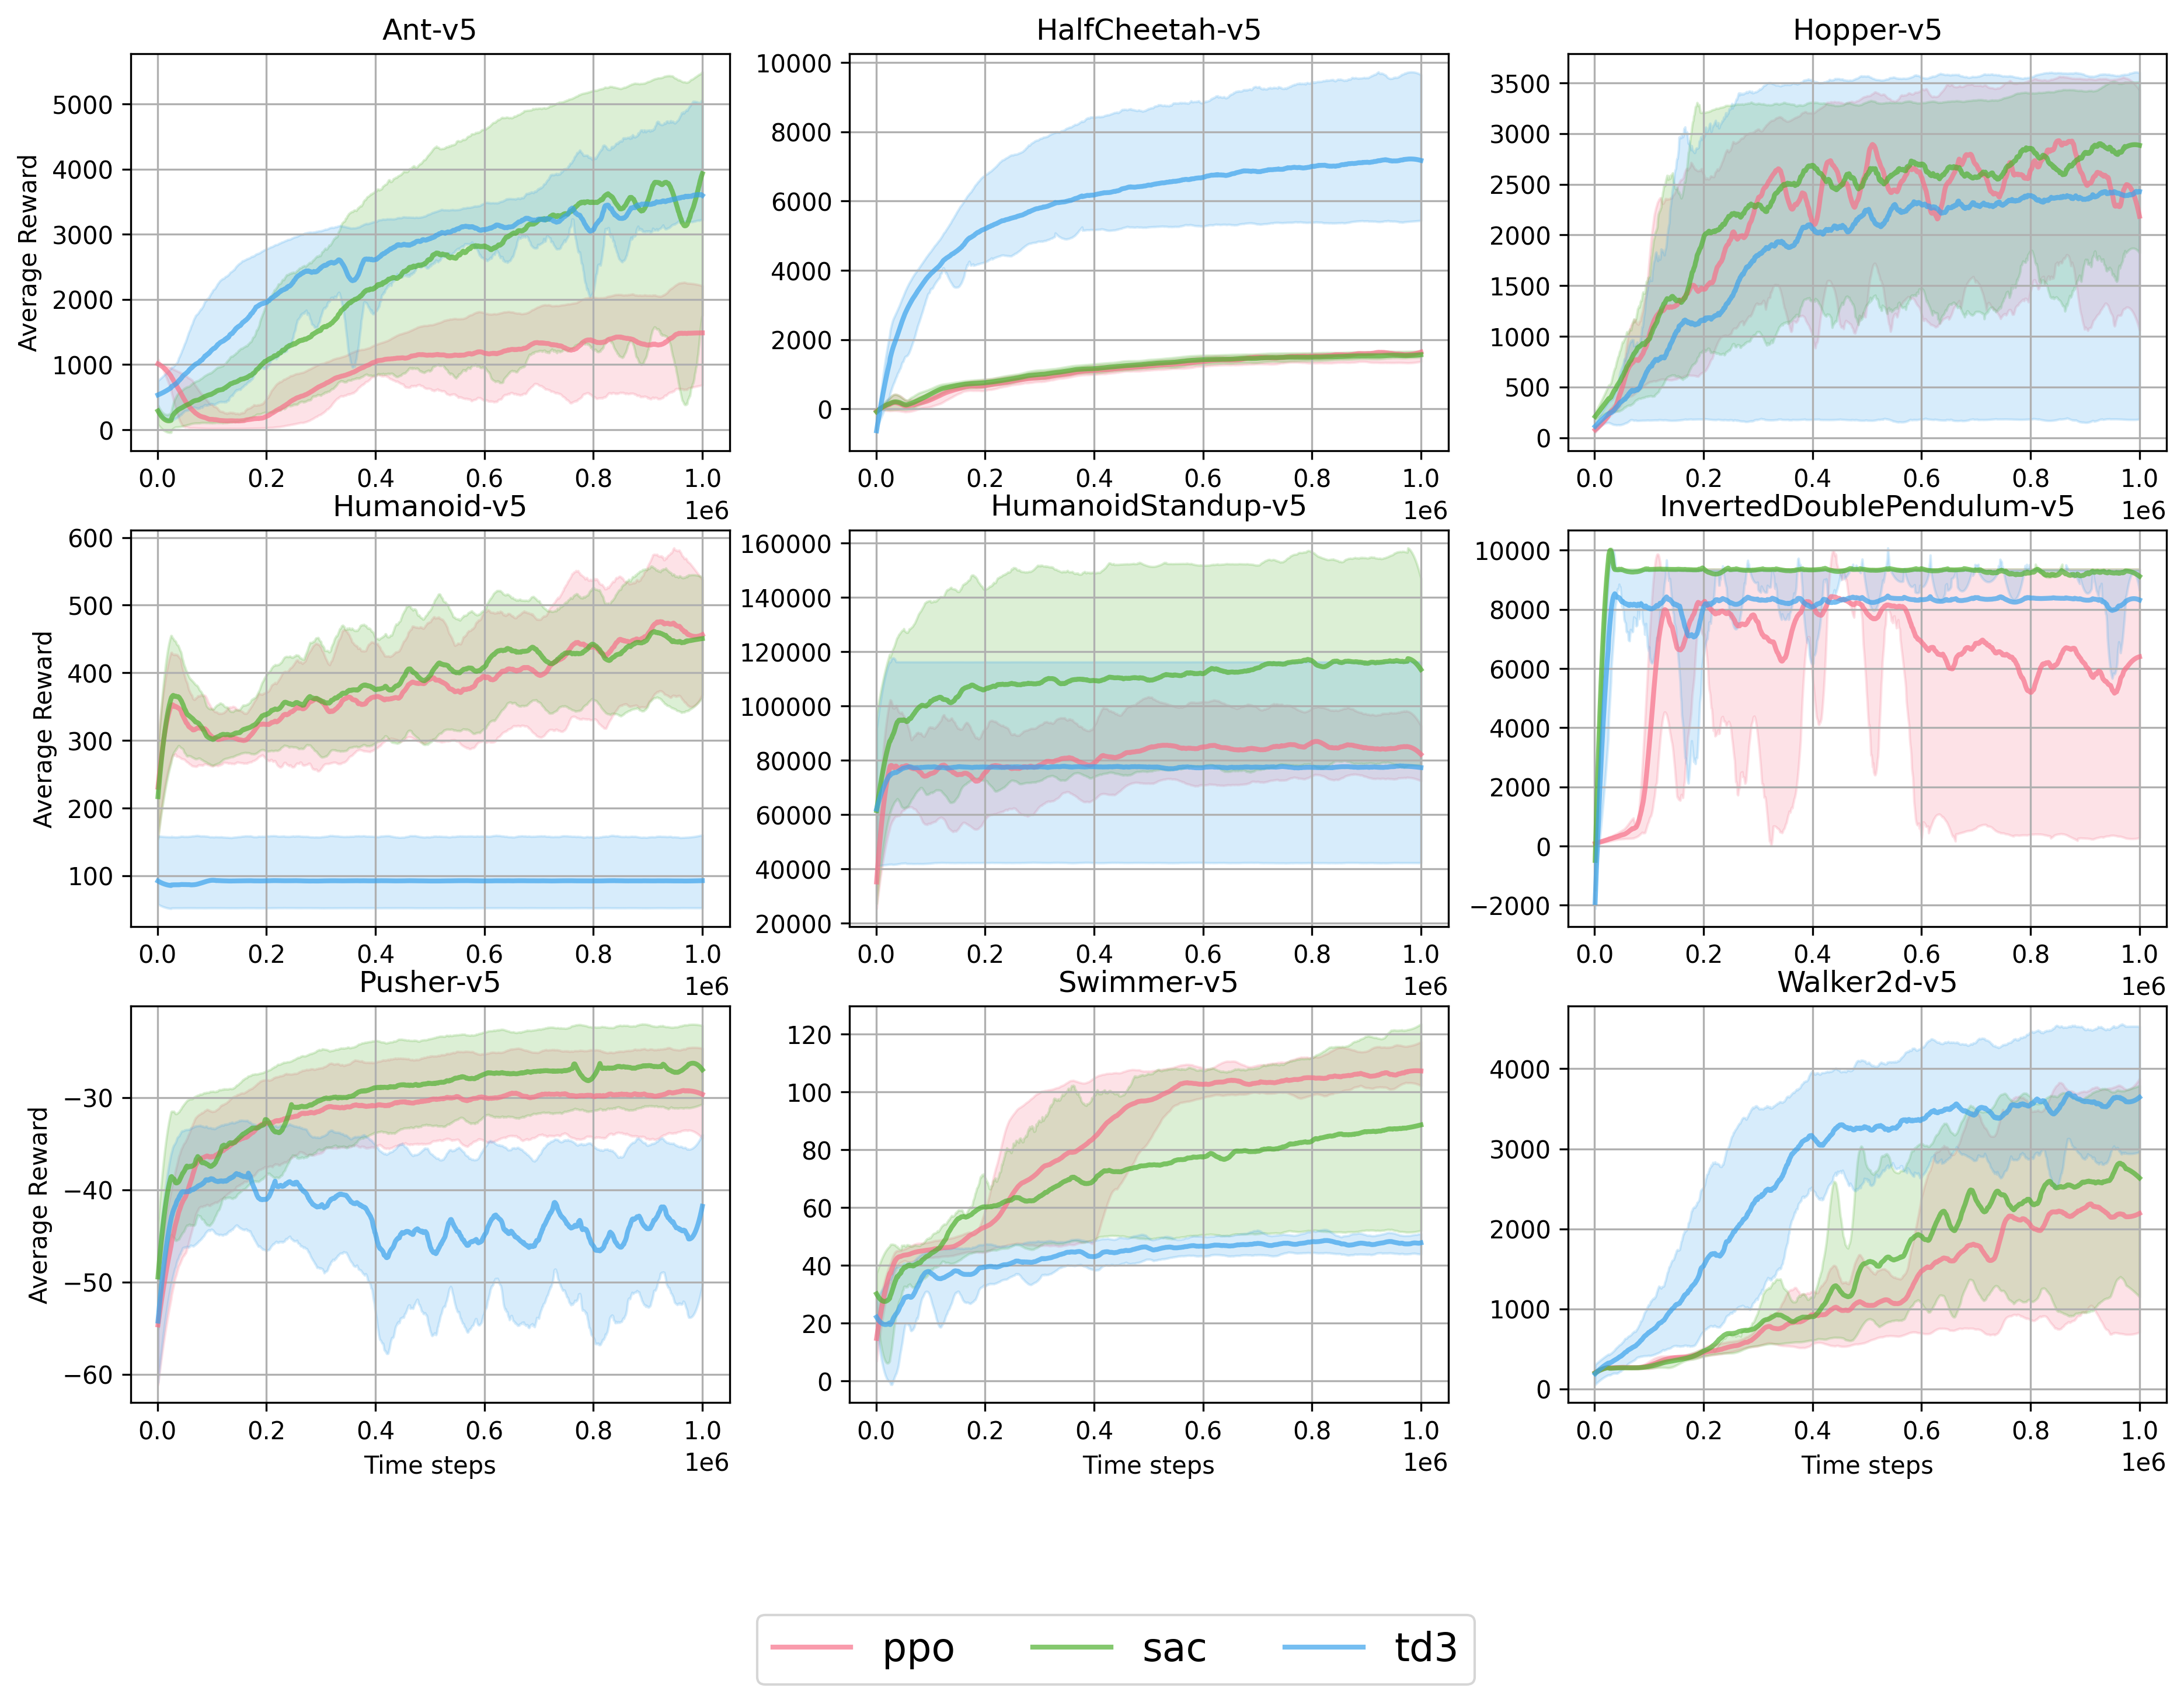
\includegraphics[width=1\textwidth]{figures/baseline_results.png}
    \caption{Sample Efficiency. The line is a smoothed average return across the 100 episodes made by each seed every 1000 times steps. The shaded area is a smoothed 70\% confidence interval highlighted }
    \label{fig:sample_efficiency}
\end{figure}

Information on the implementations of the algorithms and the hyperparameters can be found in appendix \ref{C:appendixA}. We see across the algorithms that the newer algorithms outperform the older algorithms in both sample efficiency (how steep the line is) and asymptotic performance (the maximum value of the line). It can be be seen that REDQ and TQC both outperform SAC even though they have the same foundations.

We can see that the newest algorithms are performing the best. Particularly CrossQ performs very well on the more complex environments like Humanoid and HumanoidStandup. It is also observed that CrossQ variance is a lot larger than the other algorithms which is most stark in the HumanoidStandup environment. This is likely due to the fact that CrossQ uses layer normalization which can lead to more variance in the learning process.

\textit{State how well sunrise has done.}

\dots

\subsection{Computational Efficiency}

The measure of computational efficiency is about measuring the amount of computation it takes to get a an agent to learn a certain task. As there is a variety of different algorithms the mos general method is to measure the wall clock time it takes the algorithm to complete a certain number of environment steps.

\begin{figure}[H]
    \centering
    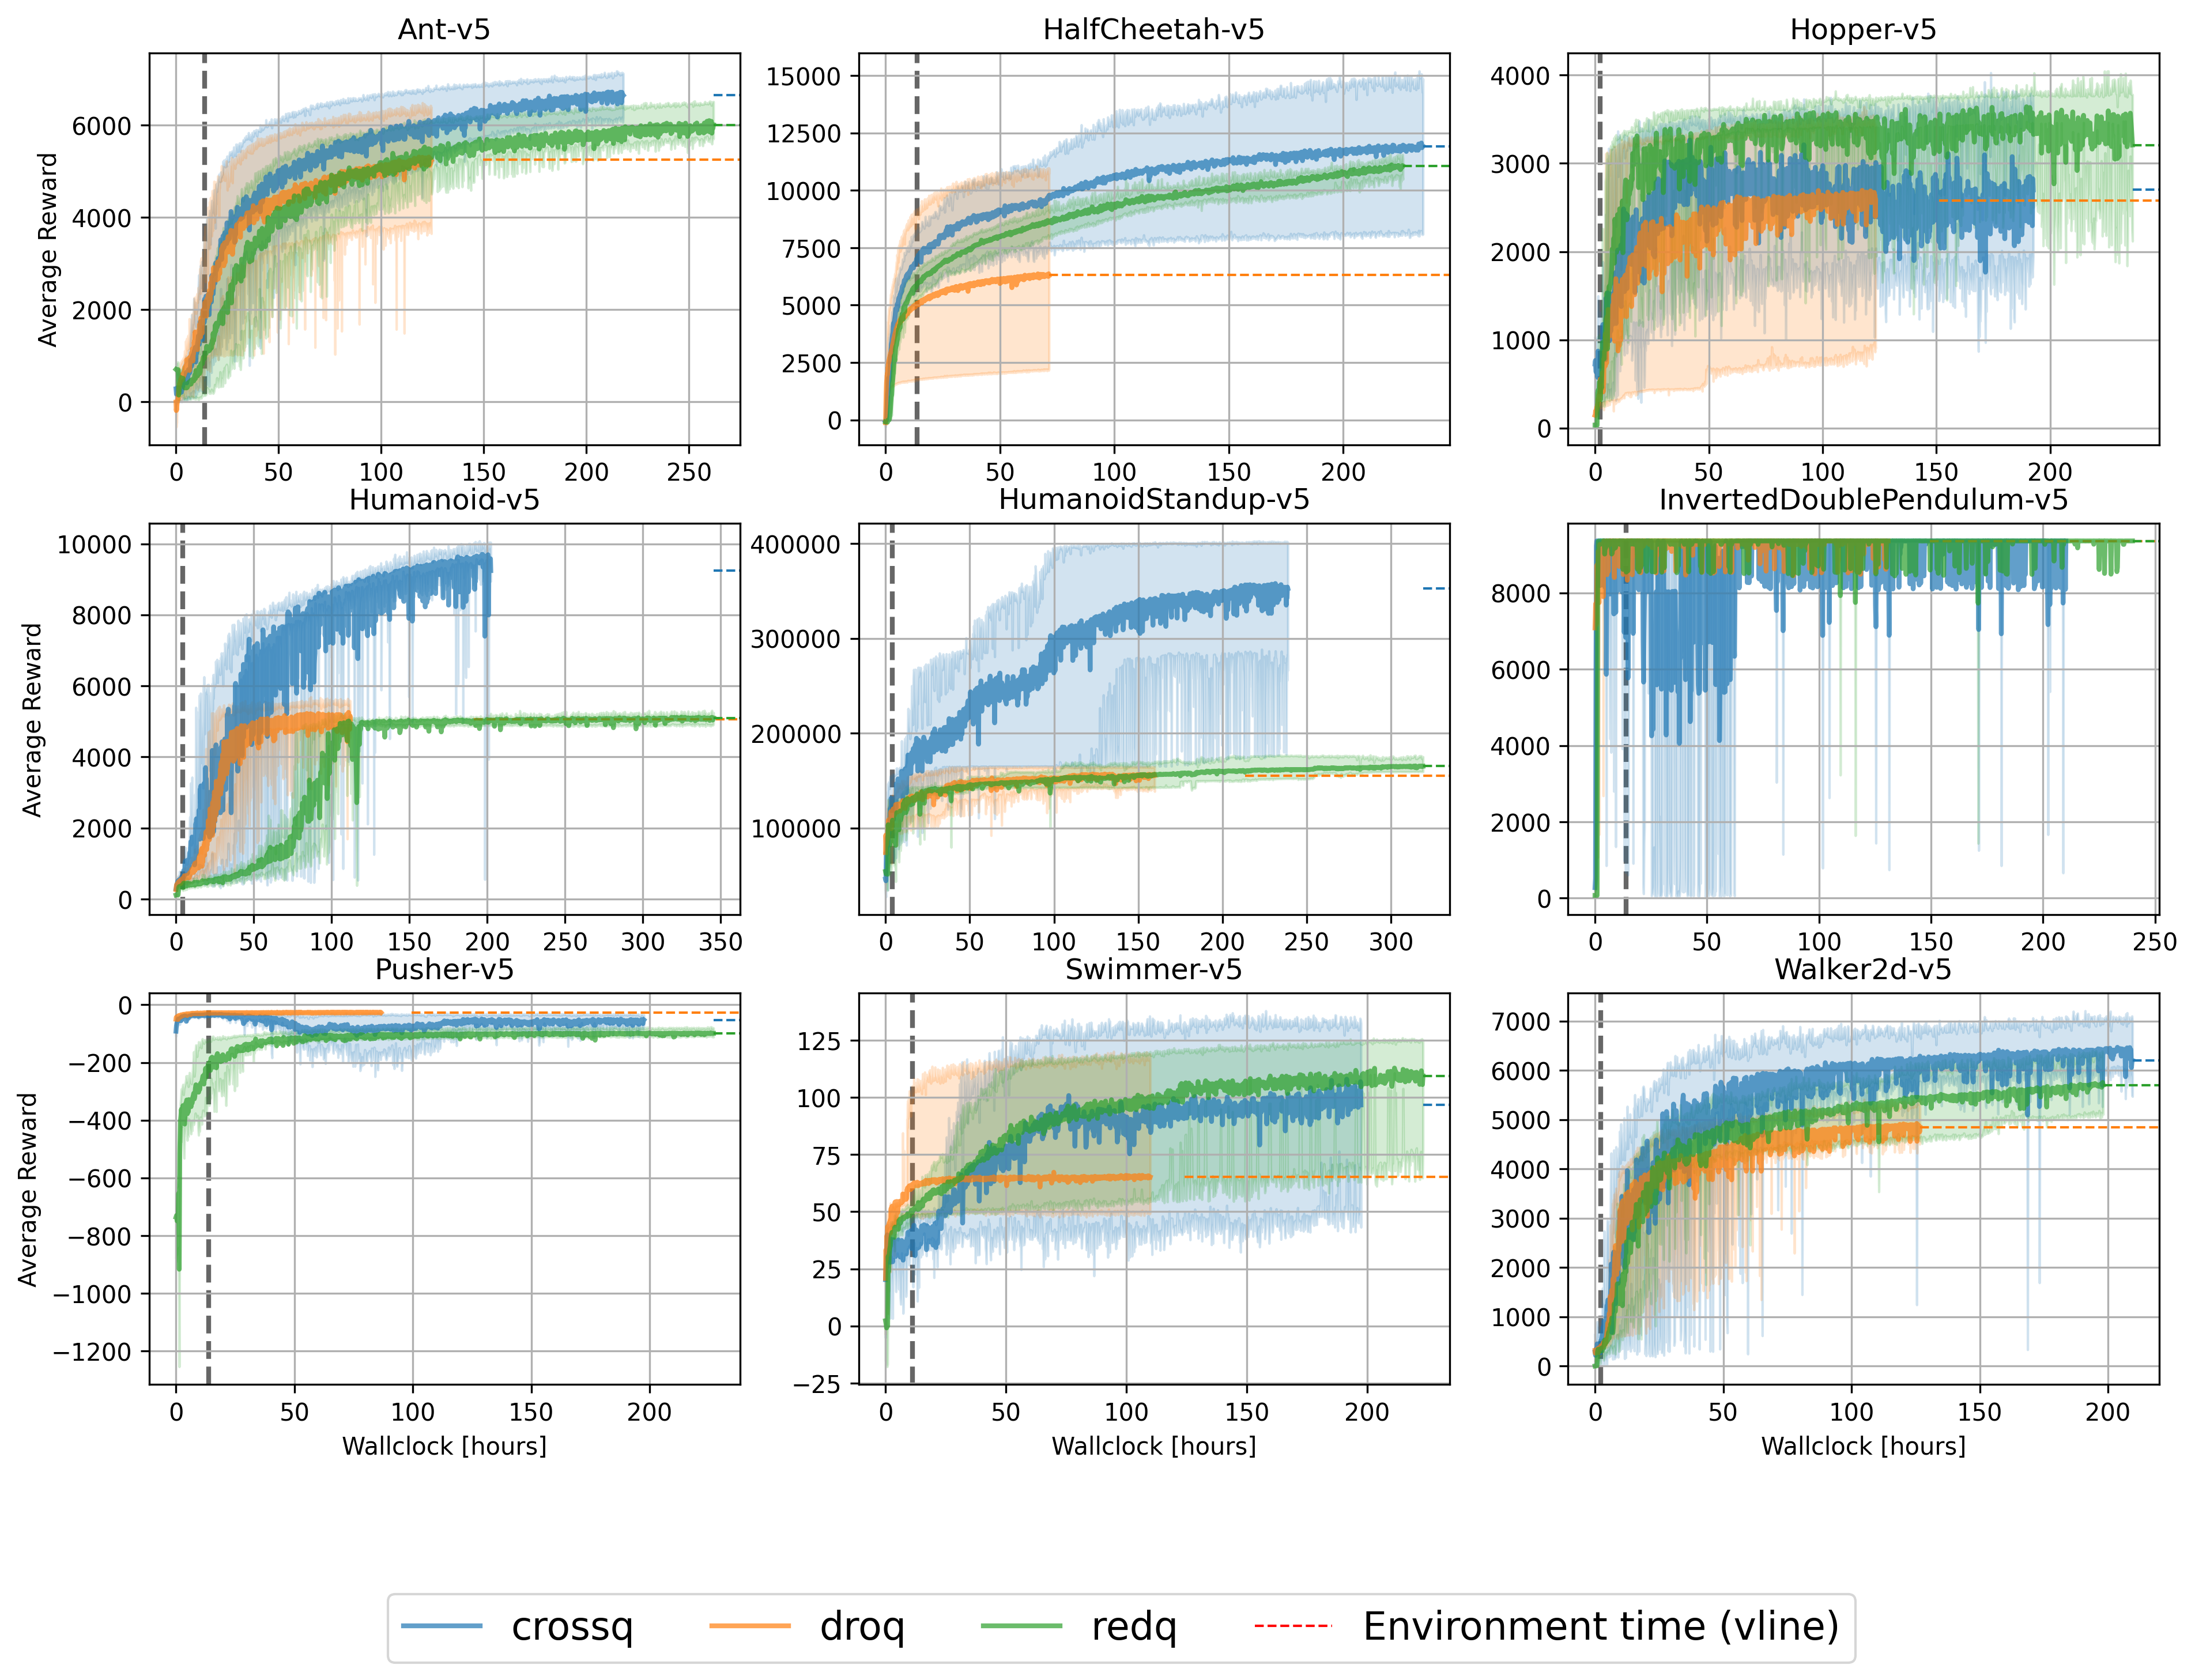
\includegraphics[width=1\textwidth]{figures/wall_clock_results.png}
    \caption{Wall clock time to get to 1 million environment time steps. Vertical lines is how long a million time-steps is in the environment. Horizontal line is the mean average reward at the end of the million steps of learning to help comparisons.}
    \label{fig:sample_efficiency}
\end{figure}

All of experiments were run on similar CPU only machines. See the appendix \ref{C:appendixA} for more information. The goal of graph is not to look at absolute time (however that is interesting to know) it is about the comparing the difference between algorithms given the same hardware.

It is interesting to note that the most modern algorithms redq and crossq are the longest running in terms of wall clock time. More importantly we can see that the method of redq having alot of critics is computationally expensive and results in a wall clock time almost 4 times that of sunrise which is also a modern ensemble method.

Looking at the horizontal lines can give us a rough idea of whether we are learning in realtime, faster than realtime or slower than realtime. We can see that for a more complicated task like HumanoidStandup we are learning significantly slower than realtime. Whereas the simpler environments are not so drastically slower than realtime. Given the hyperparameters are the same for all environments the only difference in environments is the action and state dimension as well as simulation time. Deeper analysis would have to be done to detangled the affect of simulation time and the action/state dimension in the wall clock time.

\dots

\section{Ensemble diversity}
The key idea of DSunrise is to ensure that the diversity of the ensemble of actors is maintained. As DSunrise can be directly compared to Sunrise, we can look at the diversity of the ensemble throughout training.

\begin{figure}
    \centering
    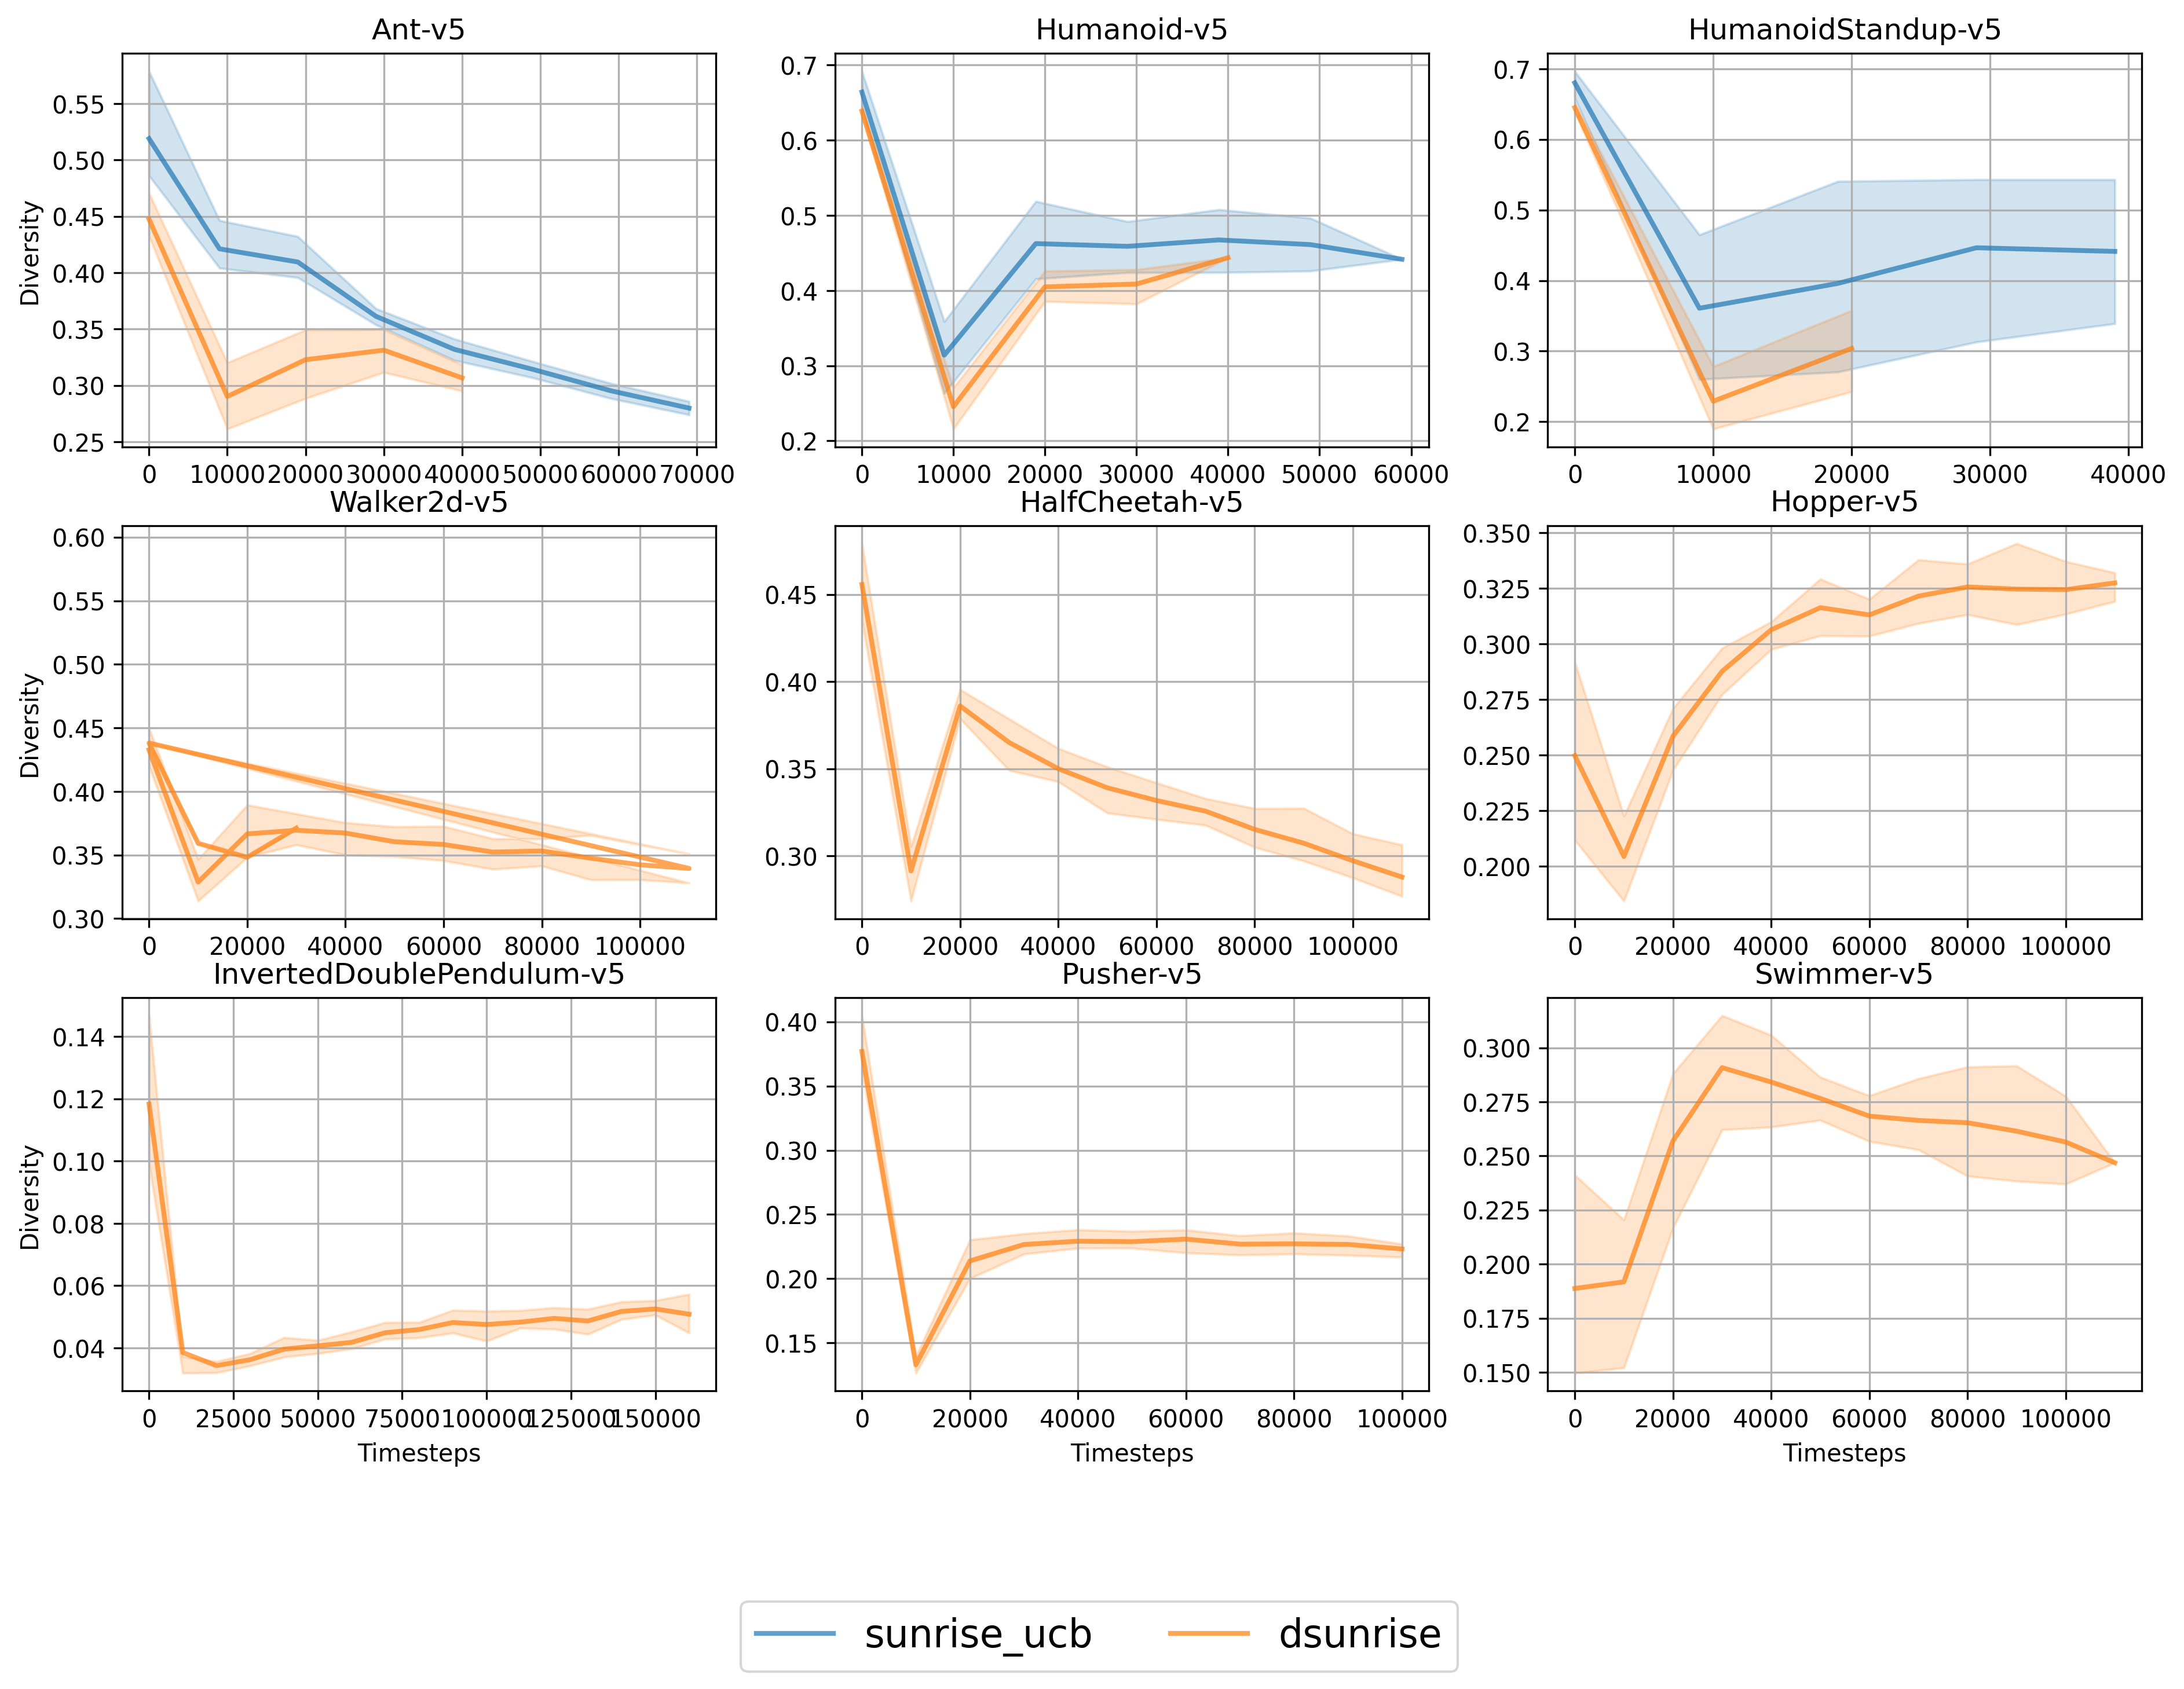
\includegraphics[width=1\textwidth]{figures/diversity_results.png}
    \caption{Diversity of the ensemble over time. The shaded area is a smoothed 70\% confidence interval highlighted.}
    \label{fig:diversity}
\end{figure}

\textit{Still waiting on the completed results for this.}

As one would expect the diversity of the ensemble decreases over time as the agents learn to do the task and converge towards the optimal policy. The goal of DSunrise is to maintain the diversity of the ensemble.

\chapter{Conclusions}\label{C:con}

Reinforcement Learning is a powerful framework for learning how to act. The recent combination of addition of deep learning has made reinforcement learning more powerful than ever. In this report I have covered the basics of reinforcement learning and the algorithms that are used to solve the problem. I have also evaluated some foundational algorithms and shown that they are capable of solving complex problems. 

There are many ways of splitting the field of reinforcement learning. The binary splits we have looked at are model based and model free, value based and policy based and on policy and off policy. However the different solutions can merge the boundary between these splits. For example actor critic methods are explicitly both value based and policy based. Below is a table which helps summarise the differences between the modern algorithms.

\begin{table}[h]
    \footnotesize
    \centering
    \renewcommand{\arraystretch}{1.4} % Increases row spacing for readability
    \begin{tabularx}{\textwidth}{p{1.3cm} X X X X}
        \hline
        \textbf{Feature} & \textbf{DQN} & \textbf{SAC} & \textbf{PPO} & \textbf{TD3} \\
        \hline
        \textbf{Algorithm type}       & Value based      & Actor-critic         & Policy based (with actor critic style)              & Actor-critic  \\
        \textbf{Policy learning}      & Off policy        & Off policy           & On policy            & Off policy    \\
        \textbf{Learnt policy}        & Deterministic     & Stochastic           & Stochastic           & Deterministic \\
        \textbf{Exploration strategy} & $\epsilon$-greedy & entropy maximisation & entropy maximisation & noise         \\
        \textbf{Action space}         & Discrete          & Continuous           & Both                 & Continuous    \\
        \textbf{Extra features} & Experience replay, ensemble Q-functions & Experience replay, ensemble Q-functions & - & Experience replay \\
        \hline
    \end{tabularx}
    \caption{Differences between modern deep reinforcement learning algorithms.}
\end{table}
These models at their time of release were all considered state of the art for model free algorithms but due to the fast moving field are now transitioning to more foundational model which the latest algorithms are building on. These new algorithms increase not just the sample efficiency but also the asymptotic performance of the algorithms. In making these gains the newer algorithms might sacrifice some computational efficiency or stability.

The state of the art deep learning algorithms also having some differences. All of the algorithms that we have looked at however are all Actor Critic based method so all are Off policy, stochastic and use entropy maximization as the exploration strategy. There are still important differences between the algorithms as seen below.

\begin{table}[H]
    \footnotesize
    \centering
    \renewcommand{\arraystretch}{1.4} % Increases row spacing for readability
    \begin{tabularx}{\textwidth}{X X X X X}
        \hline
        \textbf{Feature} & \textbf{TQC} & \textbf{REDQ} & \textbf{DroQ} & \textbf{CrossQ} \\
        \hline
        \textbf{Target networks} & \multicolumn{3}{c}{Yes} & No \\
        \textbf{Number of critics} & 5 & 10 & 2 & 2 \\
        \textbf{UTD $\gg$ 1} & No & \multicolumn{2}{c}{Yes} & No \\
        \textbf{Policy delay} & No & \multicolumn{3}{c}{Yes} \\
        \textbf{Special features} & Truncated distributional critics  & Subset of critic ensemble for critic target, Minimization for Q-target & Dropout layers, minimization for Q-target & Layer normalisation \\
        \hline
    \end{tabularx}
    \caption{Differences between state of the art reinforcement learning algorithms.}
\end{table}

These algorithms represent some of the best performing algorithms in the field that excel in either their sample efficiency, computational efficiency or stability.

There is unknown potential in the applicability of current algorithms as well as unknown power in new algorithms. Some of the current limitations of the algorithms are the sample efficiency and the stability of the algorithms. Furthermore there is the larger problem of generalization, which is getting an agent to act intelligently on varied environments that it has never seen before with minimal to no new training.

The field of reinforcement learning is still in its infancy and there is much to be discovered. The combination of deep learning and reinforcement learning has opened up many possibilities and the future is bright and exciting.



%%%%%%%%%%%%%%%%%%%%%%%%%%%%%%%%%%%%%%%%%%%%%%%%%%%%%%%

\backmatter

%%%%%%%%%%%%%%%%%%%%%%%%%%%%%%%%%%%%%%%%%%%%%%%%%%%%%%%


%\bibliographystyle{ieeetr}
\bibliographystyle{acm}
\bibliography{AIML440}

\appendix

\chapter{}\label{C:appendixA}

\section{Experiment details}

All of the experiments were run using the same gymnasium version 1.1.1 using all of the version 5 environments. The environments were run using the default Mujoco settings. The source code for the different algorithms can be seen in the table below:

\begin{table}[H]
\centering
\caption{Source code for the different algorithms.}
\label{tab:sourcecode}
\begin{tabular}{l|c}
\toprule
\textbf{Algorithm}                & \textbf{Source Code}             \\
\midrule\midrule
SAC, PPO, DQN and TD3 & Stable baselines3 \cite{stable-baselines3} \\

TQC & My own updated copy of the authors implementation \cite{thompson1jamesthompson1Tqc_pytorch2025} \cite{SamsungLabsTqc_pytorchImplementation} \\
REDQ & My own copy of the authors implementation \cite{thompson1jamesthompson1REDQ2025} \cite{watchernyuWatchernyuREDQ2025} \\
DroQ and CrossQ & Using SBX which is part of Stable Baselines 3 \cite{stable-baselines3} \\
Sunrise & My own updated copy of the authors implementation \cite{thompson1jamesthompson1Sunrise2025} \cite{leePokaxpokaSunrise2025} \\
DSunrise & My own implementation of the algorithm built off Sunrise code. \cite{thompson1jamesthompson1Sunrise2025} \\
\bottomrule
\end{tabular}
\end{table}

The experiments were run across multiple computers CPUs by using a grid computing facility at the School of Engineering and Computer Science at Victoria University of Wellington as well as the Raapoi HPC system \cite{RapoiClusterDocumentation}. The timed experiments were all run on Raapoi with CPU only. The CPUs are AMD EPYC Zen 3 models. The effect of the slightly different CPU speeds is mitigated as the 10 seeds will be run across a variety of CPU models. All experiments except dsunrise were run with only 2 CPU threads per job and about 10gb of memory (slightly higher for more complex environments like Humanoid). dsunrise was run on 6 CPU threads and more memory in an attempt to speed up the training process. It has little effect on the computational speeds.

The code used to run the experiments can be found at: \url{https://github.com/1jamesthompson1/AIML440_code}. With further discussion of source code in section \ref{sec:new_algorithm_source_code}.

\section{Experiment hyper-parameters}

The hyper-parameters fro the different algorithms were all taken from the respective authors original implementation. No additional hyperparameter tuning was done.

The first table shows the hyperparameters for the older deep learning algorithms \ref{tab:old_hyperparameters} and the second table shows the hyperparameters for the state of the art deep learning algorithms \ref{tab:sota_hyperparameters} the last table is for Sunrise and the new algorithm proposed.

\begin{table}[H]
\centering
\caption{Learning Hyperparameters for modern deep learning algorithms.}
\label{tab:old_hyperparameters}
\begin{tabular}{l|c|c|c}
\toprule
\textbf{Parameter}                &  SAC  & TD3  & PPO \\
\midrule\midrule
Discount Factor ($\gamma$)        & \multicolumn{3}{c}{$0.99$}             \\ \midrule
Learning Rate (Actor \& Critic)   & $0.0003$ & $0.001$ & $0.0003$\\ \midrule
Replay Buffer Size                & \multicolumn{3}{c}{$10^6$}             \\\midrule
Batch Size                        & $256$ & $100$ & $64$      \\\midrule
Activation Function               & \multicolumn{2}{c|}{\texttt{relu}}  & \texttt{Tanh}   \\\midrule
Critic Width                      & $256$ & $400$ and $300$ & $64$      \\\midrule
Critic Depth                      & \multicolumn{3}{c}{$2$}      \\\midrule
Actor Width                       & $256$ & $400$ and $300$ & $64$   \\\midrule
Actor Depth                       & \multicolumn{3}{c}{$2$}    \\\midrule
Optimizer                         & \multicolumn{3}{c}{\texttt{Adam}}     \\\midrule
Target Update Rate ($\tau$)       & \multicolumn{2}{c|}{$0.005$} & \texttt{N/A}       \\\midrule
Learning start delay              & 100 & $1000$ & \texttt{N/A}  \\\midrule
Update-To-Data ratio (UTD)        & \multicolumn{3}{c}{$1$}      \\ \midrule
Policy Delay                      & $1$  & $2$ & $1$      \\\midrule
Number of  Critics                & \multicolumn{2}{c|}{$2$}  & $1$  \\\midrule
Algorithm Specific Parameters     & \texttt{N/A} & $\begin{matrix}\text{target policy clip}=0.5\\\text{target policy noise}=0.2\end{matrix}$ & $\begin{matrix}\text{n epochs}=10\\\text{gae-}\lambda=0.95\\\text{evironment steps}=2048\\\text{clip range}=0.2\end{matrix}$ \\\midrule
\bottomrule
\end{tabular}
\end{table}

\begin{table}[H]
\centering
\footnotesize
\caption{Learning Hyperparameters for sota deep learning algorithms.}
\label{tab:sota_hyperparameters}
\begin{tabular}{l|c|c|c|c}
\toprule
\textbf{Parameter}            &  TQC & REDQ  & DroQ & CrossQ\\
\midrule\midrule
Discount Factor ($\gamma$)        & \multicolumn{4}{c}{$0.99$}             \\ \midrule
Learning Rate   & $0.001$ & $0.0003$ & $0.003$  & 0.003          \\ \midrule
Replay Buffer Size                & \multicolumn{4}{c}{$10^6$}           \\\midrule
Batch Size                        & \multicolumn{4}{c}{$256$}               \\\midrule
Activation Function               & \multicolumn{4}{c}{\texttt{relu}}     \\\midrule
Critic Width                      & $512$ & $256$ & $256$ & $2048$      \\\midrule
Critic Depth                      & $3$ & \multicolumn{3}{c}{$2$}      \\\midrule
Actor Width                       & \multicolumn{4}{c}{$256$}   \\\midrule
Actor Depth                       & \multicolumn{4}{c}{$2$}    \\\midrule
Target Update Rate ($\tau$)       & \multicolumn{3}{c|}{$0.005$}         & \texttt{N/A}  \\\midrule
Adam $\beta_1$                    & \multicolumn{3}{c|}{$0.9$}           &  $0.5$  \\\midrule
Learning start delay              & 256 & \multicolumn{2}{|c|}{$5000$} & \texttt{N/A}  \\\midrule
Update-To-Data ratio        & $1$  & \multicolumn{2}{c|}{$20$} & $1$     \\ \midrule
Policy Delay                      & $1$  & \multicolumn{2}{c|}{$20$} & $3$     \\\midrule
Number of  Critics                & $5$  & $10$ & \multicolumn{2}{|c}{$2$} \\\midrule
Algorithm Specific     & $\begin{matrix}\text{n quantiles}=25\\\text{dropped quantiles}=2\end{matrix}$& $\begin{matrix}\text{sampled critics}=2\\\text{initial entropy}=0.2\end{matrix}$ & $\begin{matrix}\text{dropout}=0.01\\\text{Layer normilisation}\end{matrix}$ & $\begin{matrix}\text{BatchNorm}=BRN\\\text{Momentum}=0.99\\\text{BRN Warmup}=10^5\end{matrix}$ \\\midrule
\bottomrule
\end{tabular}
\end{table}

\begin{table}[H]
\centering
\footnotesize
\caption{Learning Hyperparameters for Sunrise and DSunrise.}
\label{tab:sota_hyperparameters}
\begin{tabular}{l|c|c}
\toprule
\textbf{Parameter}            &  Sunrise & DSunrise\\
\midrule\midrule
Discount Factor ($\gamma$)        & \multicolumn{2}{c}{$0.99$}             \\ \midrule
Learning Rate                     & \multicolumn{2}{c}{$0.0003$}  \\ \midrule
Replay Buffer Size                & \multicolumn{2}{c}{$10^6$}           \\\midrule
Batch Size                        & \multicolumn{2}{c}{$256$}               \\\midrule
Activation Function               & \multicolumn{2}{c}{\texttt{relu}}     \\\midrule
Critic Width                      & \multicolumn{2}{c}{$256$}  \\\midrule
Critic Depth                      & \multicolumn{2}{c}{$2$}      \\\midrule
Actor Width                       & \multicolumn{2}{c}{$256$}   \\\midrule
Actor Depth                       & \multicolumn{2}{c}{$2$}    \\\midrule
Target Update Rate ($\tau$)       & \multicolumn{2}{c}{$0.005$}  \\\midrule
Adam $\beta_1$                    & \multicolumn{2}{c}{$0.9$}   \\\midrule
Learning start delay              & $1000$ & $10000$  \\\midrule
Update-To-Data ratio              & $1$ & $1$     \\ \midrule
Policy Delay                      & $1$ & $1$     \\\midrule
Ensemble start size               & $3$  & $10$ \\\midrule
Actor temperature                 & $0$  & $0$ \\\midrule
Critic temperature                & $20$  & $20$ \\\midrule
Bernoulli mean                    & $0.5$  & $0.5$ \\\midrule
UCB exploration                   & True & True \\\midrule
Algorithm Specific     & \text{N/A} & $\begin{matrix}\text{diversity\_threshold}=0.2\\\text{diversity\_critical\_threshold}=0.1\\\text{performance\_gamma}=0.99\\\text{window\_size}=1000\\\text{noise}=0.1\\\text{retrain\_steps}=0\\\text{removal\_check\_frequency}=10,000\\\text{removal\_check\_buffer\_size}=10,000\end{matrix}$ \\\midrule
\bottomrule
\end{tabular}
\end{table}

\section{Source code}
\label{sec:new_algorithm_source_code}

This project involved a non-trivial amount of code to conduct the various baseline experiments and to implement the new algorithm. As mentioned in the experiments appendix for a few of the modern algorithms I used my own fork which was used to update the original code to work with the latest version of gymnasium and MuJoCo. These forks will be omitted from this discussion due to their triviality. The only code that is discussed here is the code that was used to run the experiments and the code that was used to implement the new algorithm DSunrise.
\subsection{Experiment code}
The experiment code is available at \url{https://github.com/1jamesthompson1/AIML440_code}. This repository has two sections that may be of interest. 

Firstly is the \texttt{running-baseline-experiments} directory. This contains the bash and python scripts that were used to run all but the DSunrise experiments. The scripts are designed to be run on a grid computing system. Particularly run as inner scripts to a \texttt{slurm.sl} script that is called by a batch job. The scripts are then called by \texttt{slurm.sl} and passed the \texttt{SLURM\_ARRAY\_TASK} and extra parameters. The \texttt{slurm.sl} script also defines the OUTPUTDIR which is where the results of the experiments are saved. There is also a \texttt{results.ipynb} notebook that is used to process the results of the experiments and generate the figures in the report. \textit{These submission scripts and results notebooks are not designed to be used by anyone else and are specific to my experiment and cluster setup. However I believe they would still be of interest to anyone wanting somewhere to start.}

Secondly is the \texttt{my-algorithm-implementation} directory. None of the implementations in these directories were finished as each ran into enough roadblocks to prevent completion.

The \texttt{snac} directory contains the implementation of the Soft n Actor Critic algorithm. The \texttt{SNAC} algorithm was a novel algorithm that was designed to extend the SAC algorithm to use an ensemble of actors. The algorithm never reached a point of learning that was on par with some of the other modern algorithms. Therefore it was shelved in favour of other ideas that involved adapting SUNRISE. A write up to introduce the algorithm can be found here \href{https://github.com/1jamesthompson1/AIML440_report/blob/0e27a47f8df93954e2c0a70a535f7041ccb857df/my-algorithm-ideas/output/SnAC.pdf}{SnAC.pdf}.

The \texttt{SUNRISE} and \texttt{DSUNRISE} directory. Given the original authors implementation of SUNRISE was implemented with tight coupling to an very outdated version of the RLkit library I wanted to re-implement the algorithm in a standalone way. The result of the attempt can be found in the \texttt{SUNRISE} directory. The implementation is close to working but there is a bug in the code that prevents it from learning after a few thousand steps (i.e it just plateaus at just above random actions). After weeks of bug searching and fixing I decided to shelve the implementation and instead use the original authors implementation of SUNRISE.

\subsection{DSunrise code}
The code for my DSunrise implementation is found at \url{https://github.com/1jamesthompson1/dsunrise}. The code started off as a fork of the original SUNRISE implementation but has since diverged and added in a new algorithm. Due to the nature of the implementation changes to the code base are spread across many files. However the two most important files are the \href{https://github.com/1jamesthompson1/dsunrise/blob/9d3b6fd8cb65dabcea6cbca64bfc4e84f7c89b80/OpenAIGym_SAC/examples/dsunrise.py}{dsunrise.py} file and the \href{https://github.com/1jamesthompson1/dsunrise/blob/9d3b6fd8cb65dabcea6cbca64bfc4e84f7c89b80/OpenAIGym_SAC/examples/sunrise\_ensemble.py}{sunrise\_ensemble.py} file. The \texttt{dsunrise.py} file is the entry point for the DSunrise algorithm and from there calls all relevant parts of the algorithm. The \texttt{readme} file in the repository contains instructions on how to run the algorithm and how to use the code.

\end{document}
